\documentclass[12pt]{article}
\usepackage{amsmath}
\usepackage{graphicx}
\usepackage{hyperref}
\usepackage[latin1]{inputenc}
% \usepackage{exercise}
\usepackage{cancel}
\usepackage[margin=2.5cm]{geometry}
\usepackage{float}
% \usepackage{wrapfig}
% \usepackage{amssymb}
% \usepackage{subfigure}
\setlength\parindent{0pt}

\title{Computational Neuroscience - Notes}
\author{Francesco Negri}
\date{A.Y. 2022-2023}

\begin{document}
\maketitle

\tableofcontents
\newpage

\section{Introduction}
\graphicspath{ {./images/01/} }
First of all, some crucial definitions are reported in the following.
\begin{itemize}
    \item \textbf{Computational Neuroscience:} an approach to properly understand the information content of
          neural signals by modelling the nervous system at several different scales. The final goal
          is to bridge the gap between experimental observations of neuronal systems and theoretical
          models.
    \item \textbf{Model:} equations with specified parameters, generally hard to be solved
          analytically.
    \item \textbf{Simulator:} a software which is able to execute or solve a model.
    \item \textbf{Simulation:} the execution of a model into a simulator.
    \item \textbf{Reverse Engineering:} the exploitation of experimental data to build better models
          by inferring some of the parameters.
\end{itemize}
Generalized models are extremely difficult to build and solve, therefore proper simplifying
assumptions are often necessary.\\
Notice that in Computational Neuroscience three different levels of analysis do exist:
\begin{enumerate}
    \item \textit{Computational level}: the problem
    \item \textit{Algorithmic level}: the strategy
    \item \textit{Implementation level}: how it is actually done by networks of neurons
\end{enumerate}
As brain computation is distributed, it is vital to understand how neurons are intertwined and
connected together. A proper simulation should take into account signals at several distinct
scales, not only action potentials, but also LFPs, ECoG, EEG, and so on.
\begin{figure}[H]
    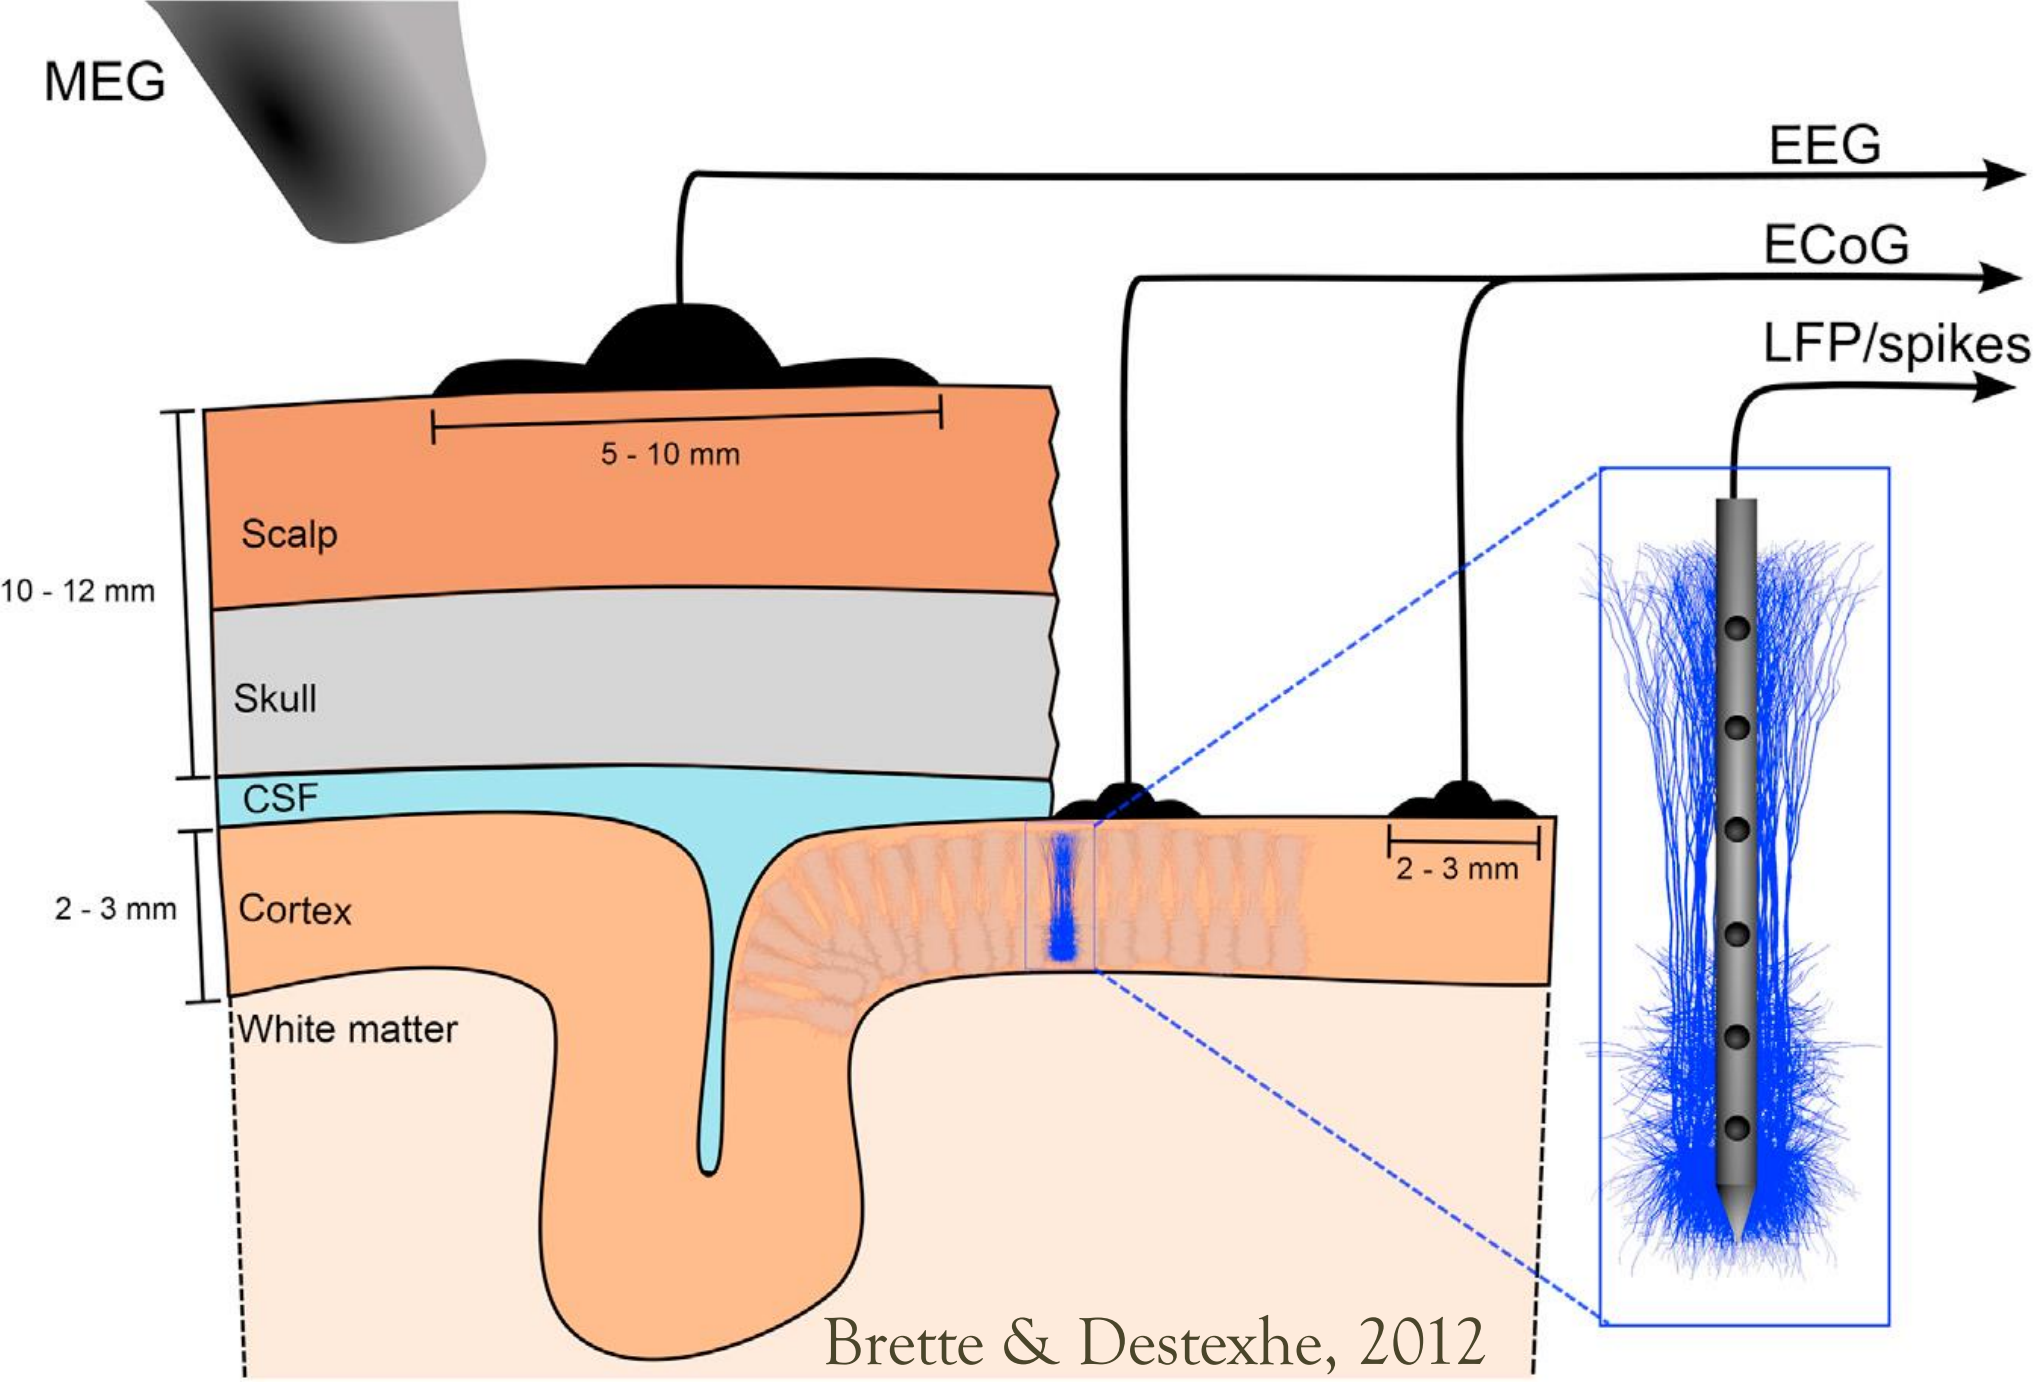
\includegraphics[scale=0.25]{01_1}
    \centering
\end{figure}
Finally, it should be stated that there is still no comprehensive theory describing information
processing in the brain, but important building blocks can be won through these approaches and
may constitute the basis for such a theory in the future.
\newpage

\section{Neuron Components and Equivalent Circuit}
\graphicspath{ {./images/02/} }
A neuron is made of several fundamental components, crucial to build a meaningful model.
\begin{itemize}
    \item \textbf{Anatomical components:}
          \begin{itemize}
              \item Soma
              \item Dendrites
              \item Axons
              \item Spines
              \item Synapses
          \end{itemize}
    \item \textbf{Biophysical components:}
          \begin{itemize}
              \item Cell membranes
              \item Ion channels (Na\({}^{+}\), Ca\({}^{2+}\), K\({}^{+}\), Cl\({}^{-}\), \dots)
              \item Receptors
              \item Transporters
          \end{itemize}
    \item \textbf{Sub-cellular components:}
          \begin{itemize}
              \item Binding proteins
              \item Calcium stores
              \item Intracellular signaling cascades
          \end{itemize}
\end{itemize}
When it comes to computational problems there are mainly two approaches nowadays.
\begin{itemize}
    \item \textit{Abstract models:} the functioning of neurons is abstracted, while their morphology
          is disregarded.
          \begin{figure}[H]
              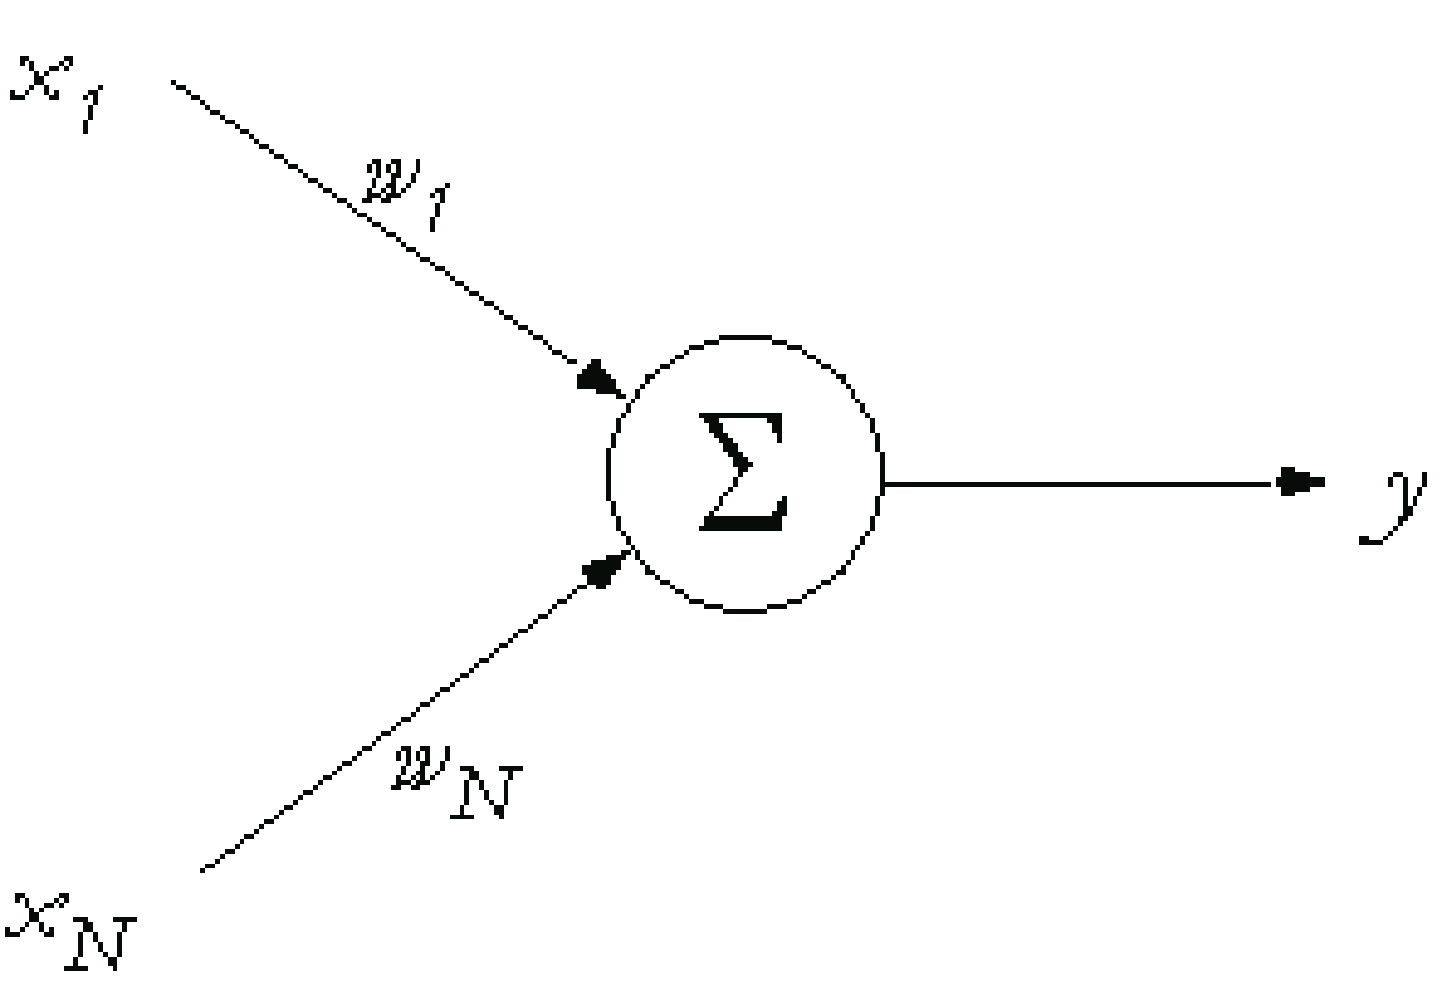
\includegraphics[scale=0.15]{02_1}
              \centering
          \end{figure}
    \item \textit{Realistic models:} the neurons morphology is kept into account as well, as it is
          considered a crucial characteristic for the model.
          \begin{figure}[H]
              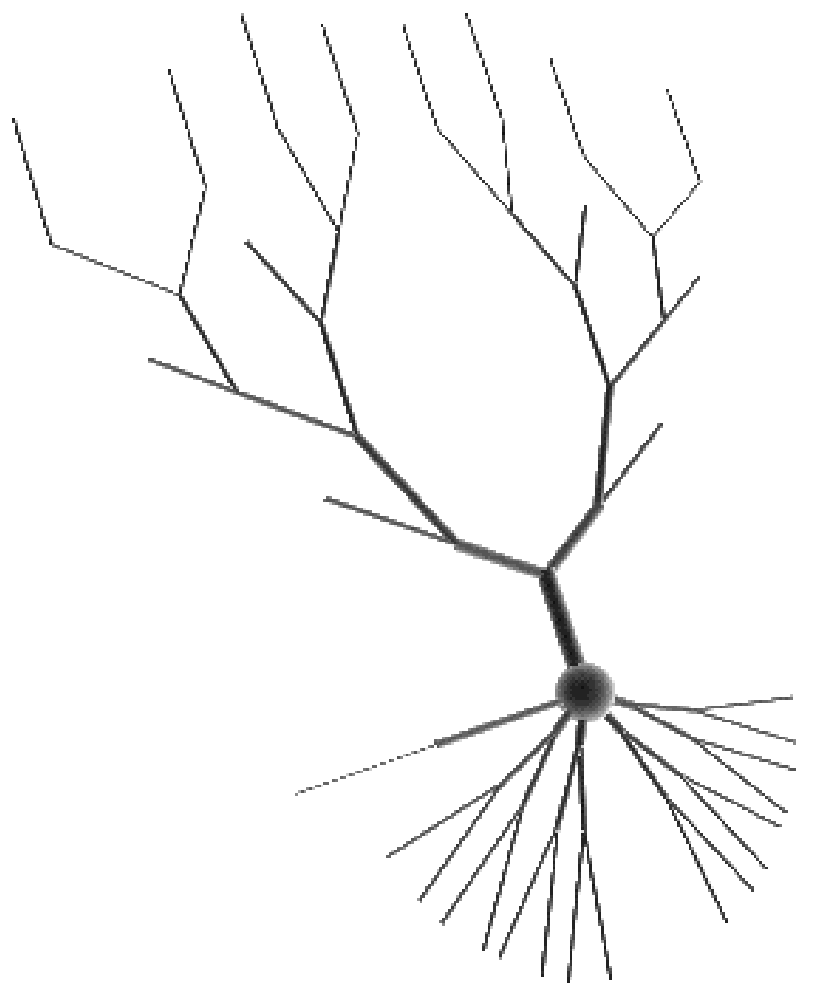
\includegraphics[scale=0.15]{02_2}
              \centering
          \end{figure}
\end{itemize}
\subsection{The Biophysical Structure of the Cell Membrane}
\paragraph{The Transmembrane Voltage}
When penetrating a neuron with a microelectrode, an electrical potential across the membrane is
measured. It is usually negative with respect to the ground (extracellular).
\begin{equation*}
    V_{m}(t)=V_{i}(t)-V_{e}(t)
\end{equation*}
The resting potential \(E_{rest}\), usually between \(-60\,mV\) and \(-70\,mV\), is the ordinary value for the
transmembrane voltage, when all the ionic currents are at the equilibrium and their net value is
zero.
\paragraph{The Transmembrane Capacitance}
A phospholipid bilayer separates the intracellular matrix from the extracellular one and it
separates ionic species, therefore it works as a capacitor, with negative charges inside the neuron
and positive charge on the outside surface:
\begin{equation*}
    Q=C_{m}\cdot V_{m}
    \hspace*{2.5cm}
    I_{C}=\frac{dQ}{dt}\Rightarrow
    I_{C}=C_{m}\frac{dV_{m}}{dt}
\end{equation*}
The membrane capacitance determines the membrane voltage dynamics, regulating how rapidly \(V_{m}\)
changes in response to a fixed current. The membrane capacitance is proportional to the surface area
of the cell, hence a specific membrane capacitance \(c_{m}\approx{1\,\mu{F}/cm^{2}}\) can be
introduced.
\paragraph{The Transmembrane Resistance}
The membrane displays voltage-independent channels with proteins allowing the leakage of ions
both into and out of the cell, iducing a current \(I_{leak}\). A leakage reversal potential
\(E_{m}\sim{E_{rest}}\) can thus be introduces. Then, the membrane voltage changes in a linear way,
following the Ohm's law:
\begin{equation*}
    V_{m}=R_{m}\cdot{I_{leak}}
\end{equation*}
where \(R_{m}\) is the transmembrane resistance. Notice that such a resistance is often
characterized by the related channel conductance \(g_{leak}=\frac{1}{R_{m}}\).\\
Holding the membrane potential steady at a level different from \(E_{rest}\) requires a certain
current, which is determined by the membrane (or input) resistance \(R_{m}\). Also in this
case it is possible to define the specific membrane resistance \(r_{m}\), independent on the
cell surface area.\\
\newline
To sum up, a neuron can be characterized by the measures reported in the picture below.
\begin{figure}[H]
    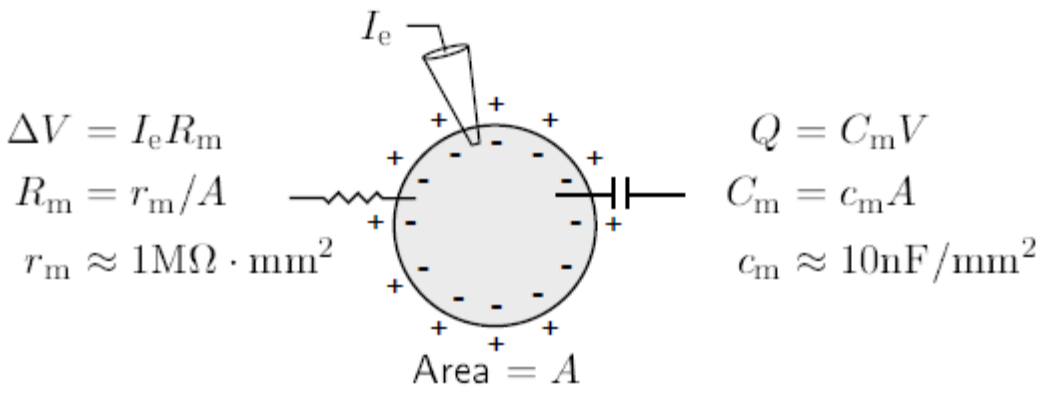
\includegraphics[scale=0.45]{02_3}
    \centering
\end{figure}
The membrane capacitance \(C_{m}\) and the membrane resistance \(R_{m}\) are employed to define
a membrane time constant \(\tau_{m}=R_{m}\cdot{C_{m}}=r_{m}\cdot{c_{m}}\) regulating the time
scale of changes in the membrane potential. It typically ranges in the \(10\,ms-100\,ms\) interval.\\
Now, the reported equivalent circuit can be derived from the previous considerations and the
relative KCL is shown just below it.
\begin{figure}[H]
    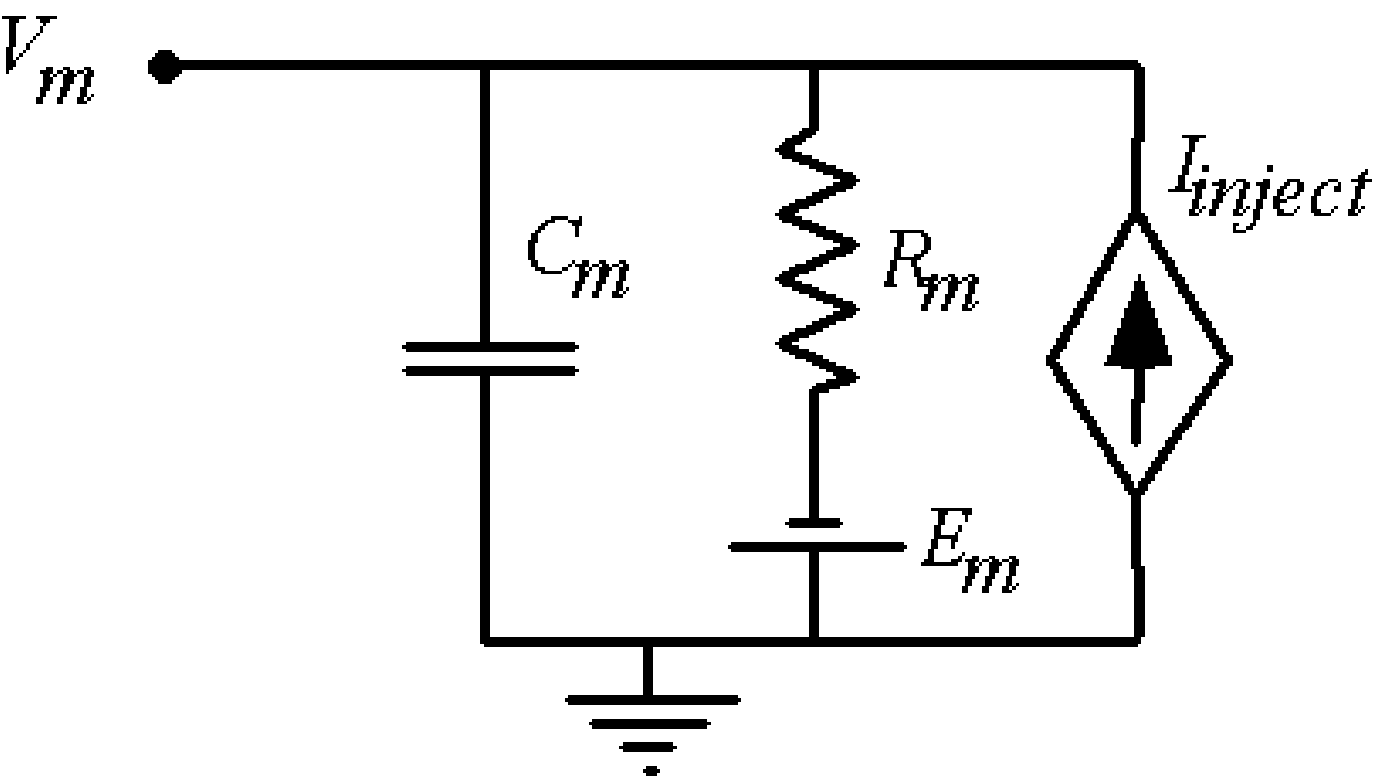
\includegraphics[scale=0.25]{02_4}
    \centering
\end{figure}
\begin{equation*}
    C_{m}\frac{dV_{m}}{dt}=-\frac{(V_{m}-E_{m})}{R_{m}}+I_{inject}
\end{equation*}
By solving the KCL, an expression for the membrane voltage as a function of time is obtained:
\begin{equation*}
    V_{m}(t)=V_{\infty}\bigl(1-e^{-\frac{t}{\tau_{m}}}\bigr)+E_{m}
\end{equation*}
\begin{equation*}
    \text{with}
    \hspace{0.25cm}
    V_{\infty}=R_{m}\cdot{I_{inject}}
    \hspace{0.25cm}
    \text{and}
    \hspace{0.25cm}
    \tau_{m}=R_{m}\cdot{C_{m}}
\end{equation*}
\subsection{Modelling the Single Channel}
So far, voltage-independent channels have been taken into account. However, cell membranes
contains a number of individual (voltage-dependent) channels. These channels open in a stochastic
way and their opening may be affected by several factors, such as the membrane potential \(V_{m}\),
intracellular ion concentration, and so on. Moreover, they are selective for one or more ions,
typically Na\({}^{+}\), K\({}^{+}\), Ca\({}^{2+}\), and Cl\({}^{-}\).
\begin{figure}[H]
    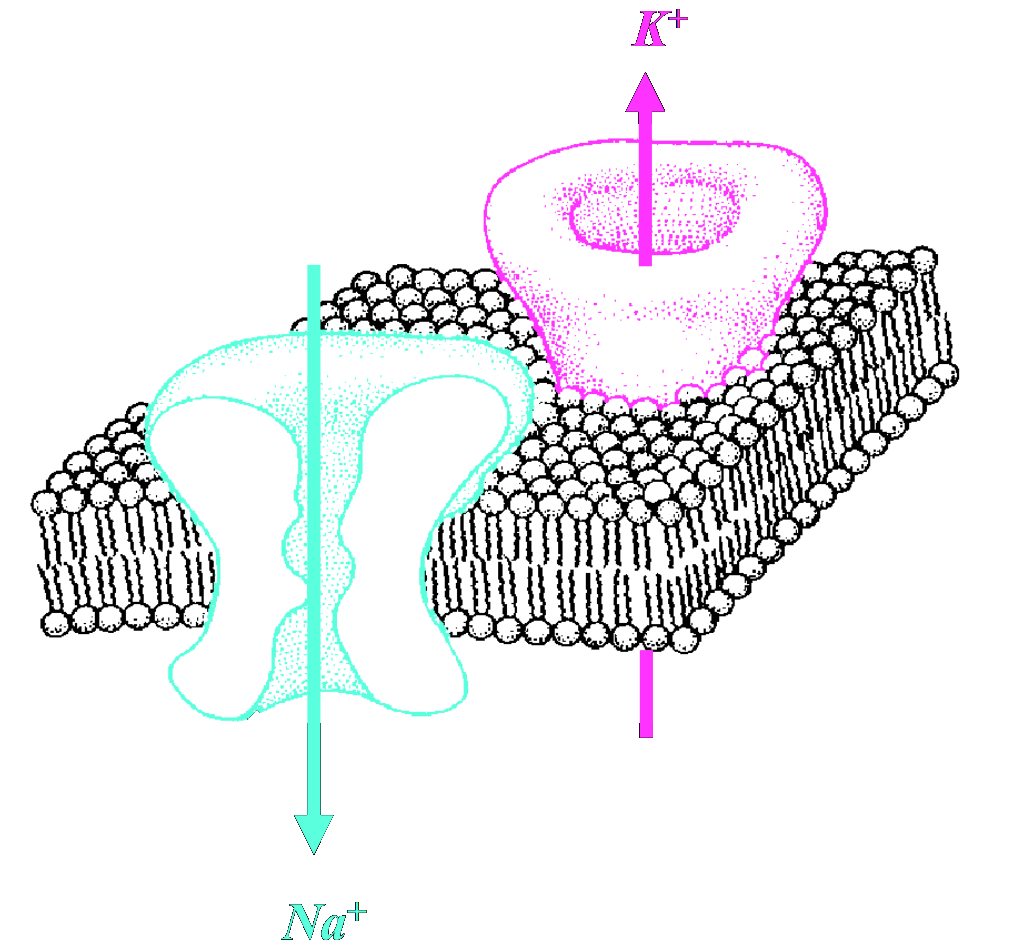
\includegraphics[scale=0.3]{02_5}
    \centering
\end{figure}
Whenever ions flow through these channels, some ionic currents \(I_{k}\) are generated. Generally,
\(I_{k}\) is related to the membrane voltage \(V_{m}\) through a linear relationship, leading
to the following equation.
\begin{equation*}
    I_{k}=g_{k}(V_{m}-E_{k})
\end{equation*}
Note that the conductance \(g_{k}\) is a function of several factors, in particular
\(g_{k}=f(V_{m},[k],t)\), with the ionic reversal potential \(E_{k}\) defined by the Nernst
equation as \(E_{k}=\frac{RT}{zF}\ln{\frac{[k]_{out}}{[k]_{in}}}\).\\
These voltage-dependent or concentration-dependent ionic currents can be incorporated in the
previously introduced equivalent circuit:
\begin{figure}[H]
    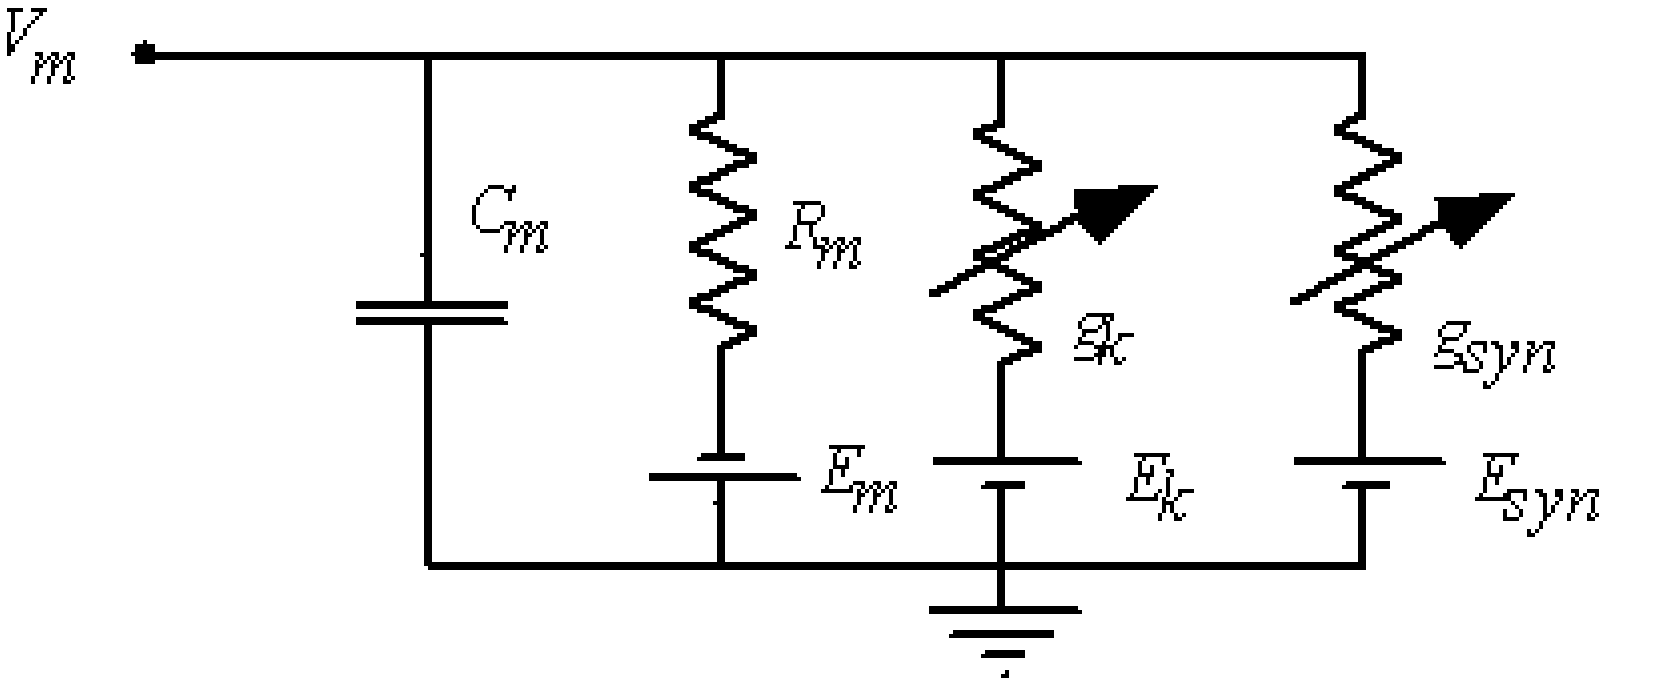
\includegraphics[scale=0.3]{02_6}
    \centering
\end{figure}
\begin{equation*}
    I_{k}=g_{k}(V_{m}-E_{k})
    \hspace{2.5cm}
    I_{syn}=g_{syn}(V_{m}-E_{syn})
\end{equation*}
Note that \(g_{syn}\) and \(E_{syn}\) are the synaptic conductance and the synaptic reversal
potential respectively.
\paragraph{Why are ionic channels modeled as resistive circuits?} The flux of ions through each
transmembrane ionic channel is ruled by both \textit{drift} and \textit{diffusion}. As a
consequence, they give birth to a drift-diffusion (ionic) current \(I_{k}\).
\begin{align*}
    I_{k}(x)
     & =I_{k,diffusion}(x)+I_{k,drift}(x)                      \\
     & =-z_{k}FD_{k}\frac{d[k](x)}{dx}+z_{k}F[k](x)\mu_{k}E(x)
\end{align*}
where \(E(x)\) is the electric field across the membrane.\\
By rearranging the equation, it can be obtained that:
\begin{equation*}
    \frac{I_{k}(x)}{\mu_{k}z_{k}F}=-\frac{D_{k}}{\mu_{k}}\frac{d[k](x)}{dx}+[k](x)E(x)
\end{equation*}
Note that due to the Einstein relationship \(\frac{D_{k}}{\mu_{k}}=\frac{RT}{z_{k}F}\), therefore:
\begin{equation*}
    \frac{I_{k}(x)}{\mu_{k}z_{k}F[k]}=
    -\frac{RT}{z_{k}F}\frac{1}{[k](x)}\frac{d[k](x)}{dx}-\frac{dV(x)}{dx}
\end{equation*}
Let's now integrate all the terms:
\begin{equation*}
    \int_{0}^{\Delta{x}}{\frac{I_{k}(x)}{\mu_{k}z_{k}F[k]}}dx=
    -\frac{RT}{z_{k}F}\int_{[k]_{in}}^{[k]_{out}}{\frac{1}{[k](x)}d[k](x)}
    -\int_{V_{in}}^{V_{out}}{dV(x)}
\end{equation*}
where \(\Delta{x}\) is the membranes thickness. At this point let's assume current density which
is constant across the membrane, such that it can be taken outside the integral.
\begin{equation*}
    I_{k}\int_{0}^{\Delta{x}}{\frac{1}{\mu_{k}z_{k}F[k]}}dx=
    -\frac{RT}{z_{k}F}\ln{\frac{[k]_{out}}{[k]_{in}}}
    -(V_{out}-V_{in})
\end{equation*}
Note that \(\int_{0}^{\Delta{x}}{\frac{1}{\mu_{k}z_{k}F[k]}}dx=R_{k}\), while
\(V_{in}-V_{out}=V_{m}\), leading to:
\begin{equation*}
    I_{k}{R_{k}}=V_{m}-E_{k}
\end{equation*}
This is the Ohm's law and this relationship has been derived without any assumption on the nature
of ionic channels or about their opening and closing dynamics.\\
Eventually, a crucial remark consists in saying that the electrophysiological properties of a
neuron are not exclusively caused by peculiar kinds of channels across its membrane. Also the
neuron morphology plays a fundamental role, thus it has to be modeled too.
\newpage

\section{Modeling Complex Neuronal Structures}
\graphicspath{ {./images/03/} }
When dealing with neurons, it must be kept in mind that there are several types of
neurons characterized by peculiar morphologies and arborizations, fundamental
to properly build an effective and reliable model.\\
To encode the structure of a neuron it is necessary to acquire images of the cell itself:
this is often done via radioactive or fluorescent markers, alternatively advanced optical
methods are often employed. Successively, the model has to be quantitatively characterized,
thus the dimensions of each cell element are measured.\\
Several softwares, such as \textit{NeuroMorpho}, were introduced to reconstruct 3D models of
neurons, allowing scientists to share them across the scientific community.

\subsection{Compartmental Models}
Generally, the morphology of the dendritic arborizations is the main attribute used to classify
neurons. Compartmental models are based on the idea that the various structures found in
a neuron can be modelled separately, then they are put together, constituting the
overall realistic and working model of the target cell.\\
In order to compartmentalize a neuron, the structure is divided into three main parts:
\begin{itemize}
    \item \textbf{Soma}: it is commonly approximated to a isopotential spheroid. the
          transition points between the soma and the dendritic tree are difficult to determine.
    \item \textbf{Dendritic Tree}: it is often modelled as a complex structure made by
          linked sequences of discrete cylinders, characterized by geometrical properties.
    \item  \textbf{Dendritic Spines}: they are the major target of synapses, making their
          modelling rather complex.
\end{itemize}
During the development of a model, it is crucial to keep in mind the following relatonships:
\begin{equation*}
    {Model\,fidelity}\propto{Amount\,of\,data}
    \hspace{2.5cm}
    {Simulation\,speed}\propto{\frac{1}{Model\,fidelity}}
\end{equation*}
An example of compartmental model is reported below, in particular the KCL and KVL for the
\(j-\)th element are shown:
\begin{figure}[H]
    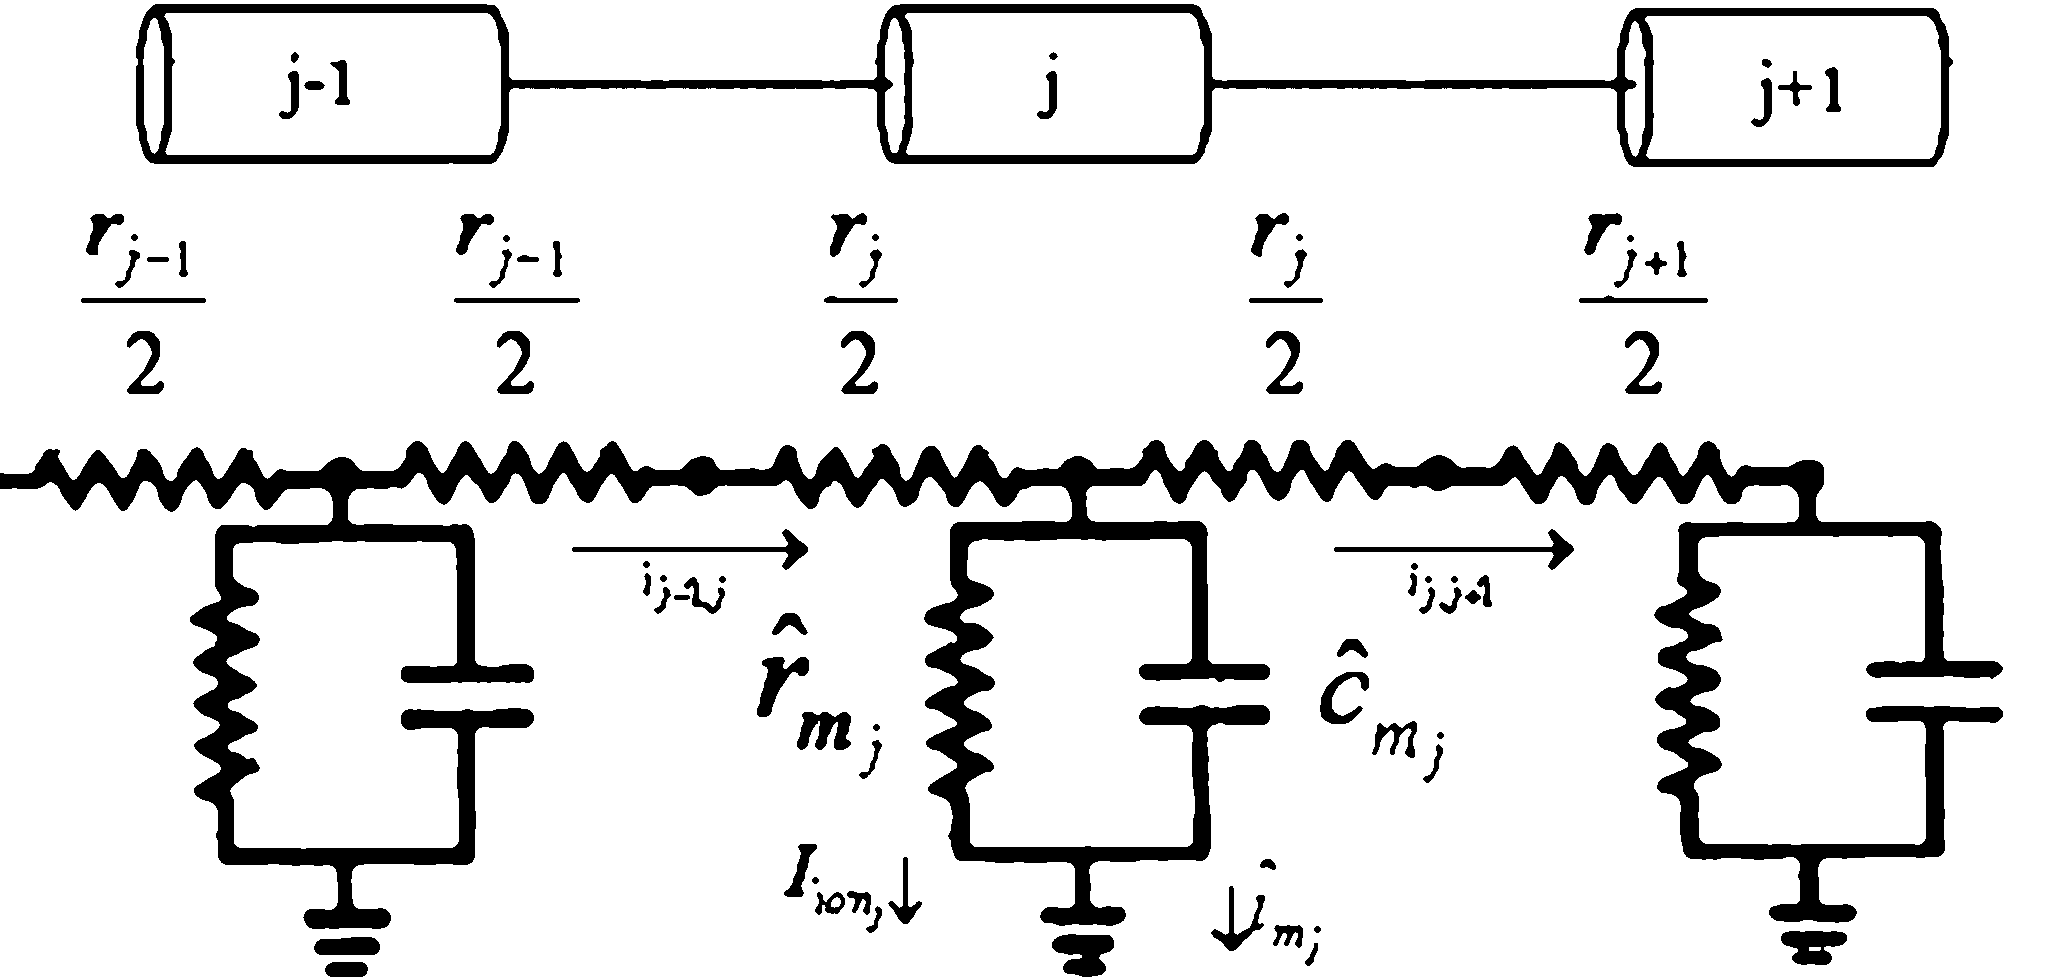
\includegraphics[scale=0.17]{03_1}
    \centering
\end{figure}
\begin{equation*}
    \begin{cases}
        \hat{i}_{m_{j}}=\hat{i}_{m_{j-1,j}}-\hat{i}_{m_{j}}=\hat{i}_{m_{j,j+1}} \\
        \hat{i}_{m_{j}}=I_{ion,j}+\hat{c}_{m}\frac{dV_{j}}{dt}+I_{stim,j}       \\
        \hat{i}_{m_{j}}=\frac{V_{j-1}-V_{j}}{r_{j-1,j}}-\frac{V_{j}-V{j+1}}{r_{j,j+1}}
    \end{cases}
    \Rightarrow
    \hat{c}_{m}\frac{dV_{j}}{dt}+I_{ion,j}+I_{stim,j}=g_{j-1,j}(V_{j-1}-V_{j})-g_{j,j+1}(V_{j}-V_{j+1})
\end{equation*}
In the equations above, \(r_{j}\) denotes the (specific) axoplasmatic resistance and \(I_{ion,j}\)
the ionic currents, including leakage and active channels, as well as synaptic contributions.
The main questions that should be answered when building a compartmental model regard the
compartmentalization criterion to employ, the estimation of the dendrites diameter if it is
not constant, and whether and how to take into account the dendritic spines. Therefore,
a segmentation (or compartmentalization) method is required.
\begin{figure}[H]
    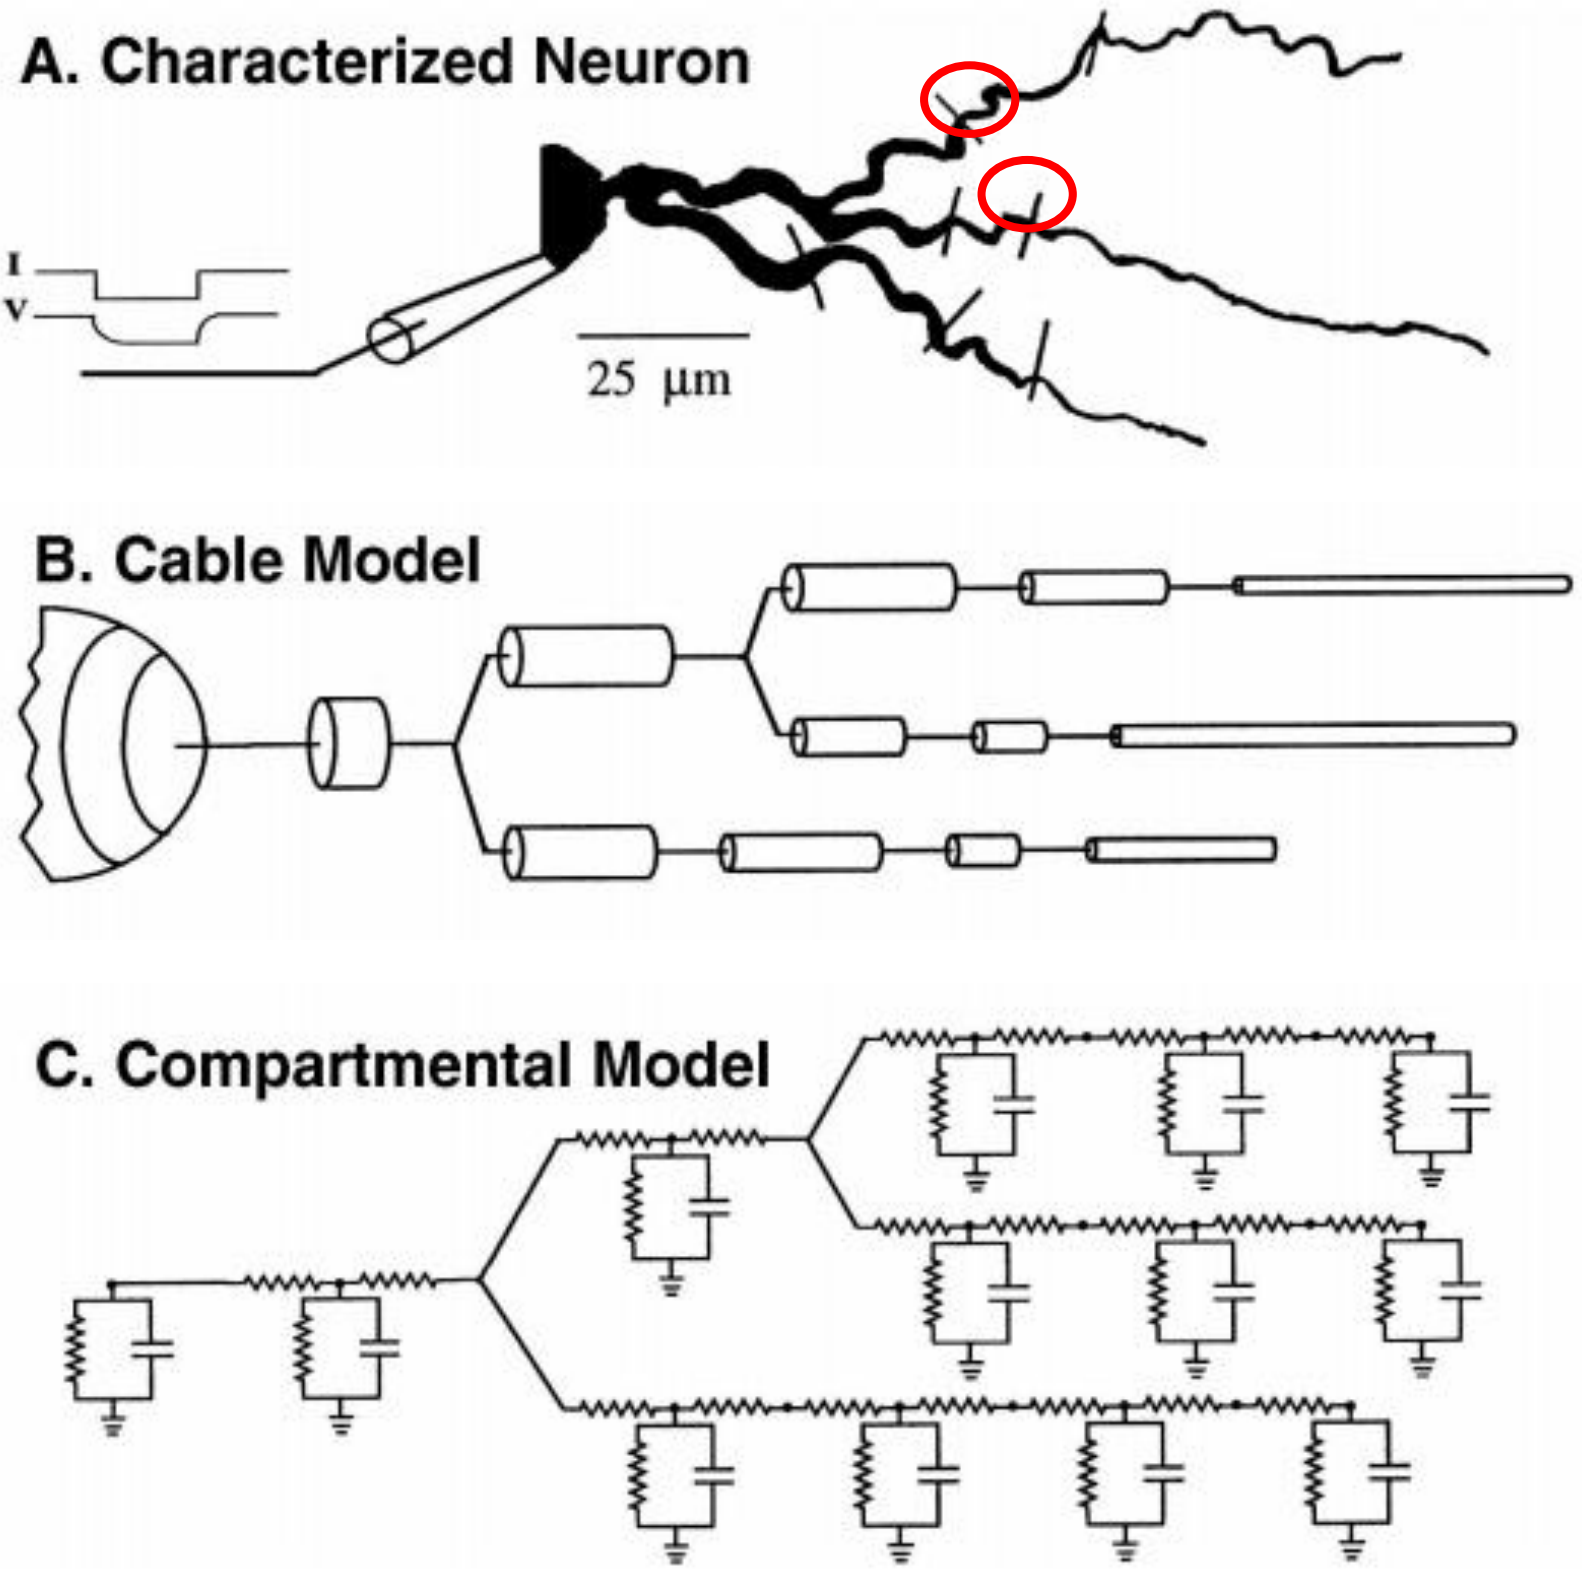
\includegraphics[scale=0.25]{03_2}
    \centering
\end{figure}
After characterizing the neuron from a geometrical point of view, a cable model, where
each dendritic segments is approximated to a cable with a specific diameter, is constructed.
Note that a threshold on the diameter is usually exploited, in order to have a discrete
set of diameters. Finally, each cable segment is considered to be isopotential and is modelled
through an equivalent electrical circuit.

\subsection{Complexity Reduction}
Given their nature, realistic and detailed compartmental models tend to be particularly
demanding from the computational point of view. Hence, the main idea is to simplify them,
losing some details in order to increase their efficiency. To do so, their level of
abstraction is increased.
\begin{figure}[H]
    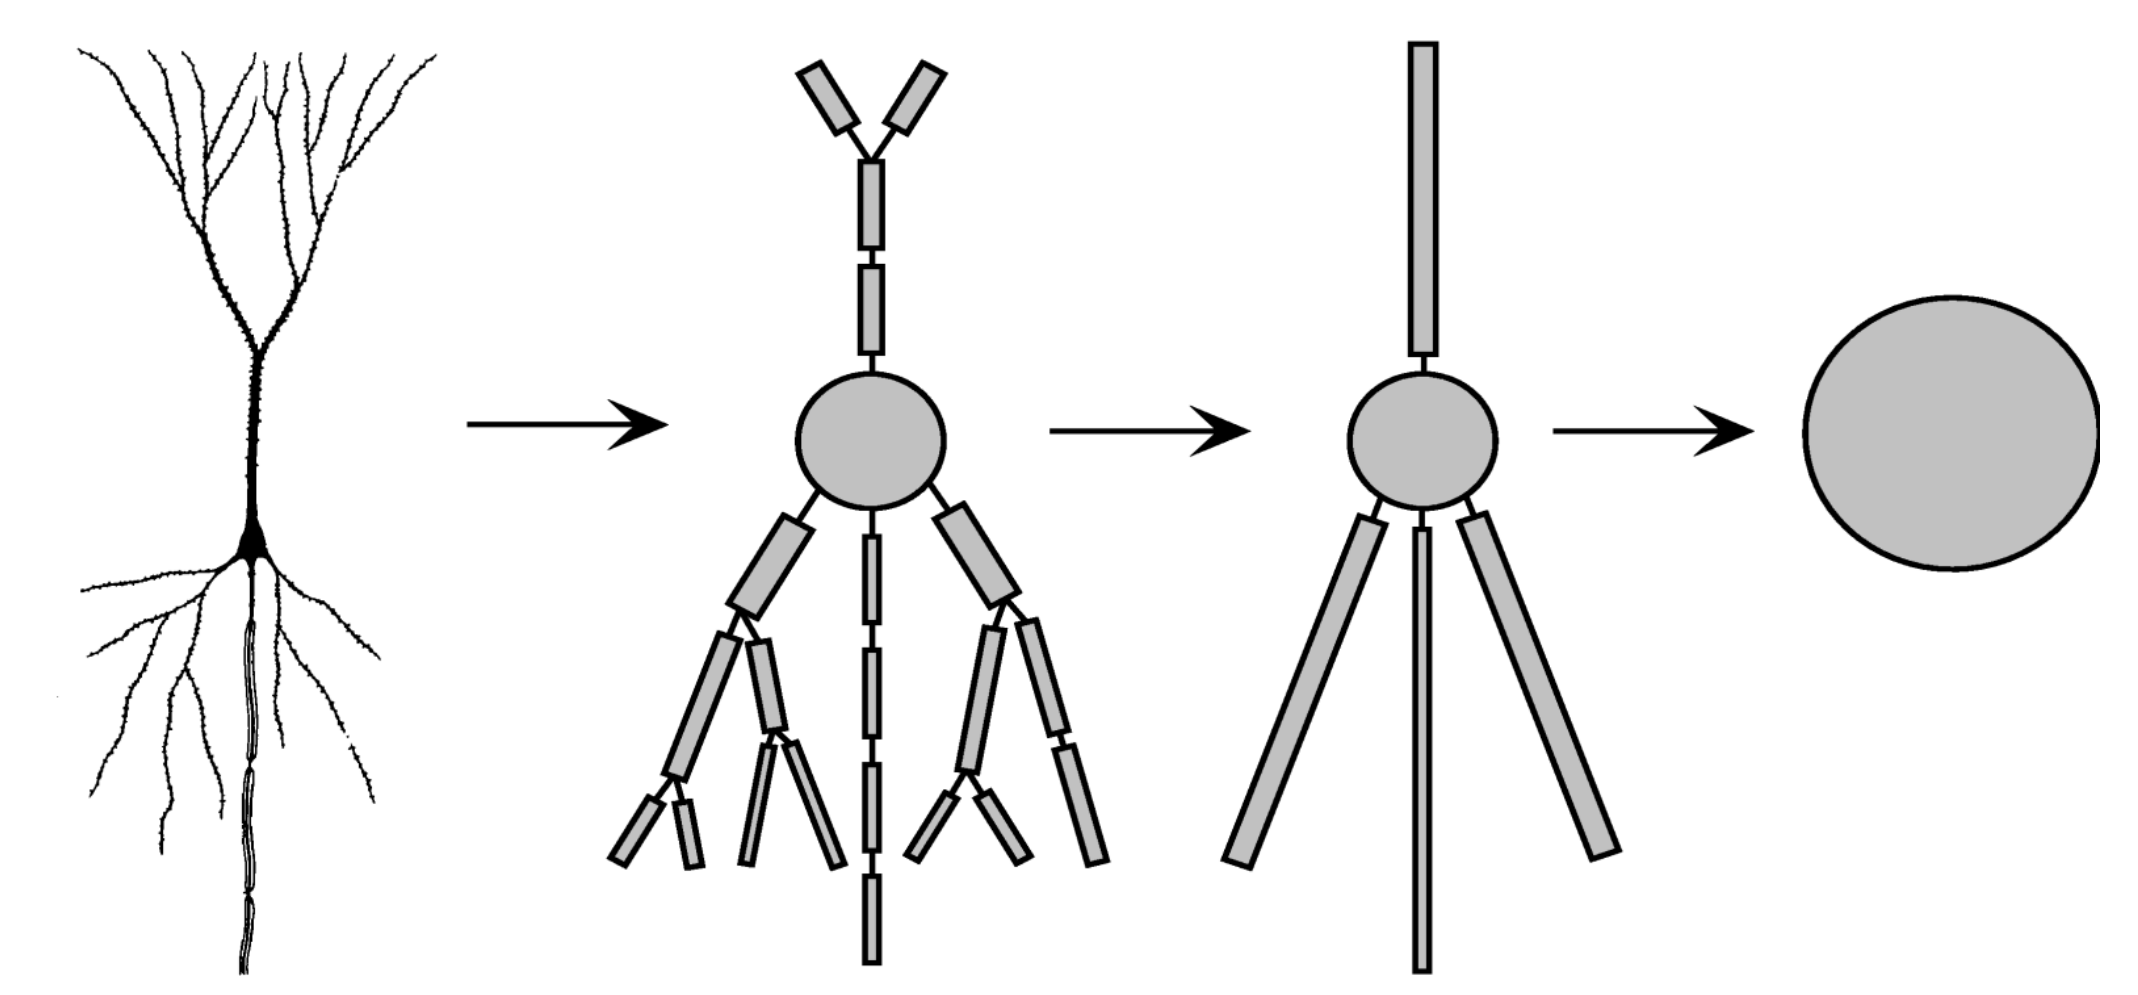
\includegraphics[scale=0.2]{03_3}
    \centering
\end{figure}
The aim is to reduce complexity while keeping the very same electrophysiological patterns,
such as bursts, spikes, and mixed activity. On the other hand, reducing a model inevitably
leads to losing certain features, ISI for instance, but it is not important as long as
these attributes are not relevant to characterize the considered model. The golden rule
when simplifying a neuronal model is that the input/output characteristic, which is
derived from stimulations, should not change. Note that the neuron spontaneous activity is
instead strictly related to the cell morphology, thus it is extremely difficult to
preserve it during model reduction.
\begin{figure}[H]
    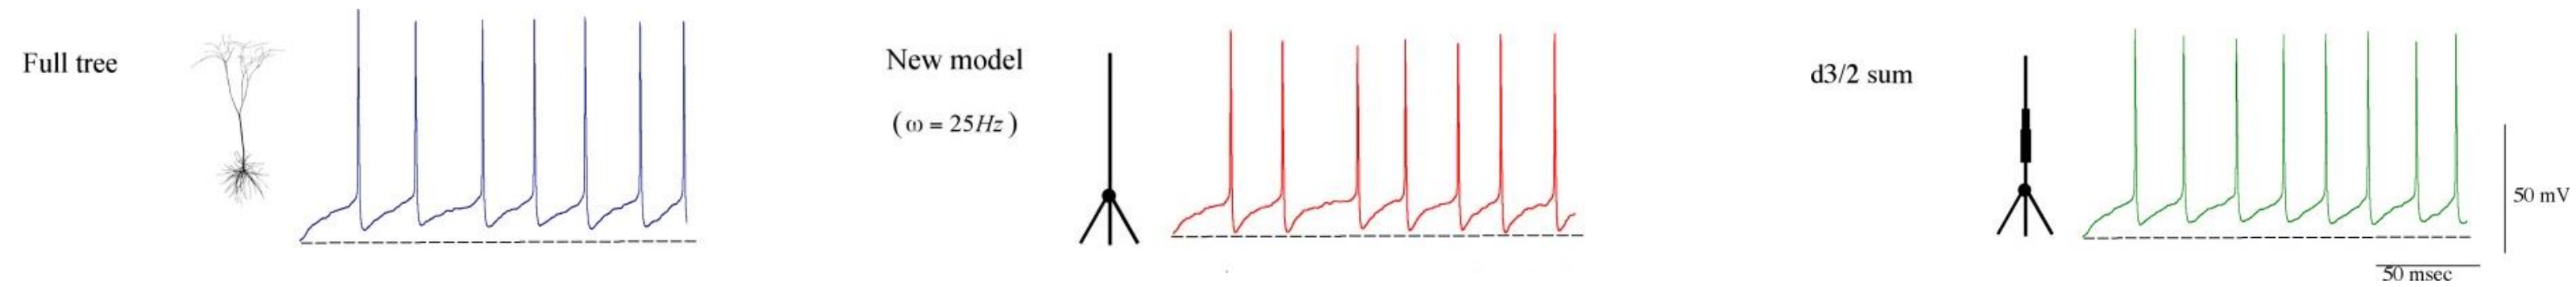
\includegraphics[scale=0.25]{03_4}
    \centering
\end{figure}
\paragraph{The Rall's Equivalent Cylinder}
The main idea is that the whole dendritic tree of a neuron can be represented as a single cylinder
having a constant diameter. In the model proposed by Rall, the soma is substituted by
a compact region (a single compartment), while the entire dendritic tree is replaced by
a single equivalent cylindrical cable. Said so, it is crucial to properly select the
geometrical and electrical properties of such a cylinder, such as its radius \(a\) and
length \(L\).
\begin{figure}[H]
    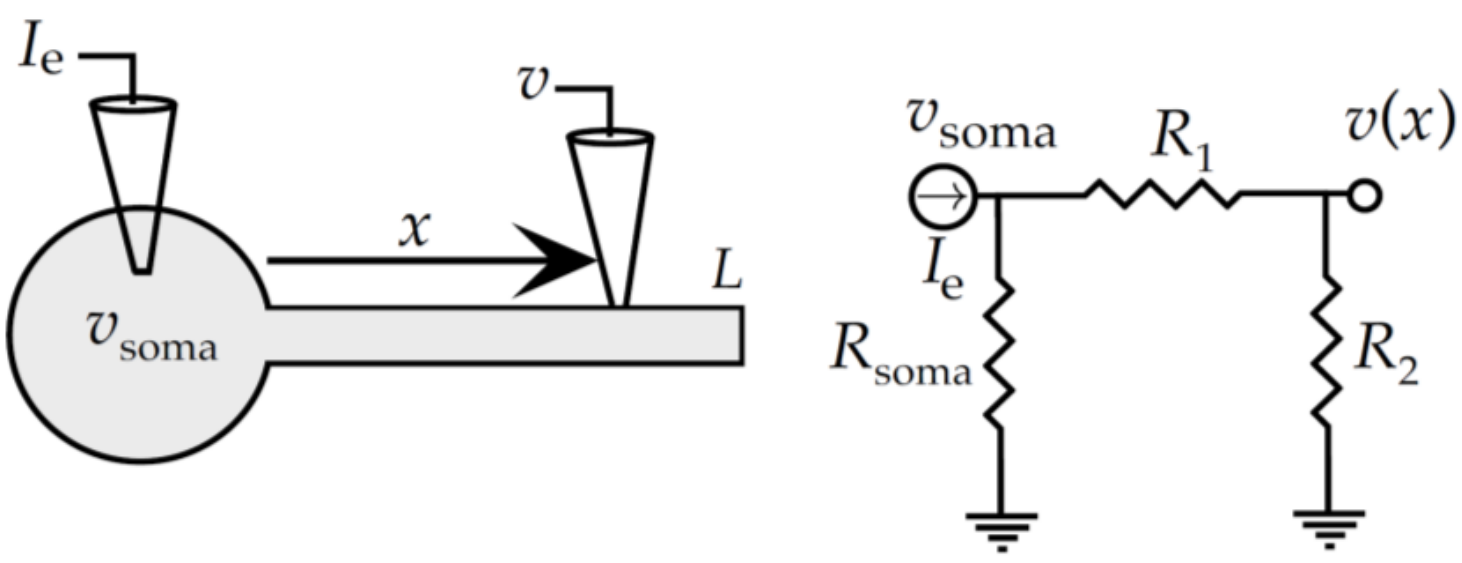
\includegraphics[scale=0.35]{03_5}
    \centering
\end{figure}
\(L\) and \(a\) are carefully selected to match two critical properties of the dendritic
tree. As a matter of fact, \(L\) is related to the average electrotonic length,
determining the degree of attenuation of the electrical input as a function of the distance.
The electrotonic length is measured by summing all the electrotonic segment lengths according
to the designated end point and then computing an average measure, describing the average
signal decay rate between the input and the output ends.\\
Differently, \(a\) is employed in the computation of the total surface area \(2\pi{a}\cdot{L}\),
crucial to correctly model the membrane resistance and capacitance of the neuron. The Rall's
model neuron input resistance \(R_{in}\) can be derived as follow:
\begin{equation*}
    R_{in}=\frac{(R_{1}+R_{2})R_{soma}}{(R_{1}+R_{2}+R_{soma})}
\end{equation*}
\begin{figure}[H]
    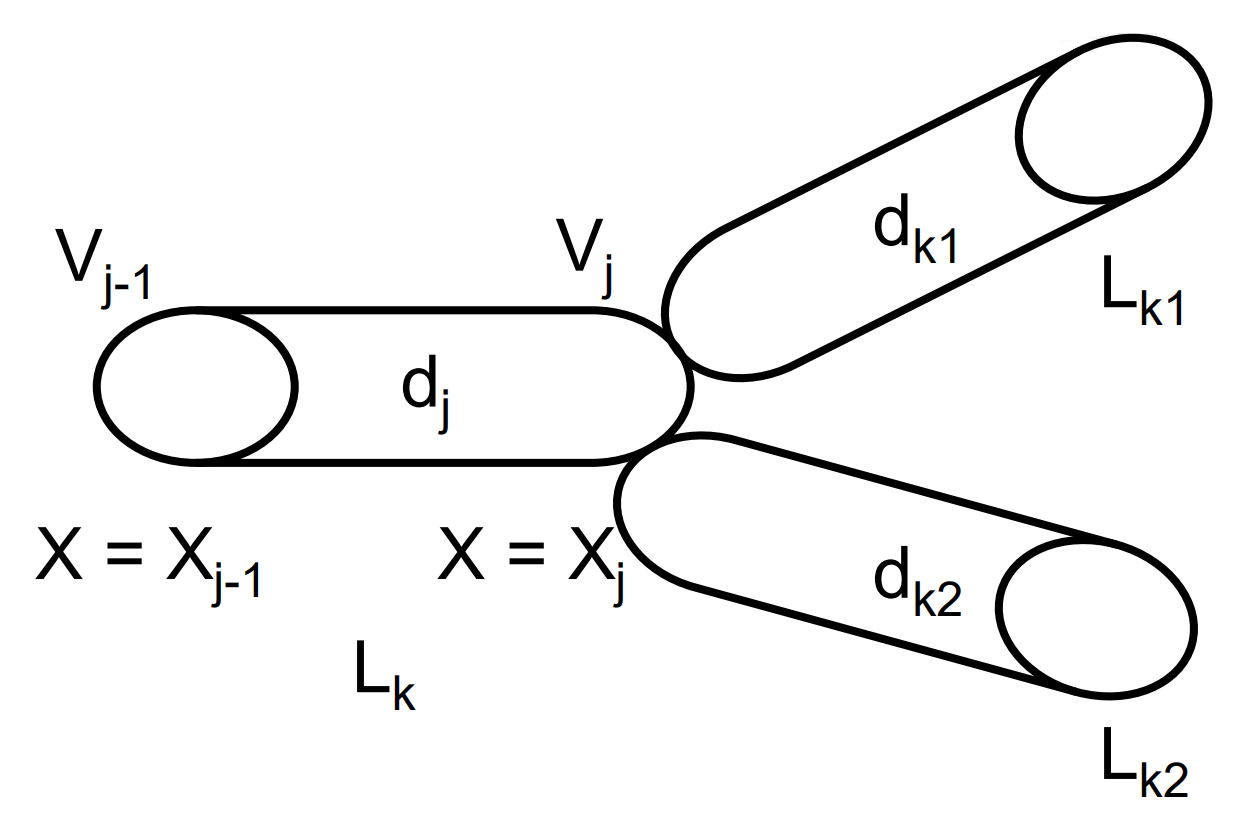
\includegraphics[scale=0.2]{03_6}
    \centering
\end{figure}
The Rall's model can be used with neurons matching three particularly strict criteria:
\begin{enumerate}
    \item The electrotonic lengths of all paths from soma to dendritic ends must be identical.
          \begin{equation*}
              L_{k}=L_{k1}=L_{k2}
          \end{equation*}
    \item The sum of the diameters of child branches at each branch point, raised to the power
          of \(\frac{3}{2}\) must equal the diameter of the parent branch, also raised to the power
          of \(\frac{3}{2}\).
          \begin{equation*}
              (d_{j})^{\frac{3}{2}}=(d_{k1})^{\frac{3}{2}}+(d_{k2})^{\frac{3}{2}}
          \end{equation*}
    \item The electrical properties should be constant and uniform as much as possible, in
          particular \(R_{m}\) and \(R_{i}\) must be spatially uniform within the branching structure.
          \begin{figure}[H]
              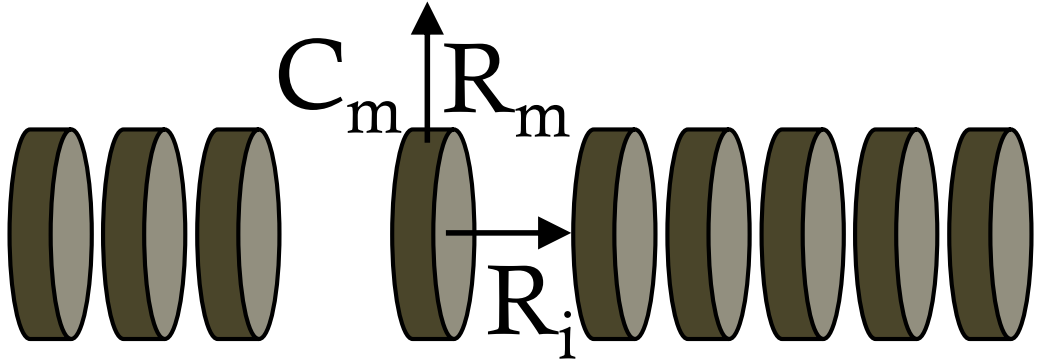
\includegraphics[scale=0.15]{03_7}
              \centering
          \end{figure}
\end{enumerate}
To sum up, the Rall's cable approach wants to substitute the whole dendritic tree with a single
cable having a constant diameter and the surface area distributed, with respect to the electrotonic
distance, similarly to the one of the original tree. Unfortunately, real neurons does not exhibit
morphological characteristics compliant with the Rall's criteria, therefore a less strict model
is to be introduced.
\paragraph{The Equivalent Cable}
This model was introduced to overcome the limitations of the Rall's cylinder, as a matter of
facts the idea is once again to model the whole dendritic tree as a single cable, but
the diameter is no longer assumed constant: it changes as a function of distance. This allows
a modelling much more precise in terms of electrical quantities, since they are strictly
related to the radius of the equivalent cable. A parameter \(\Delta{x}\) regulates the degree
of detail of the model, in particular it represents the length of a segment with constant
diameter of the overall cable. A very small \(\Delta{x}\) generates an extremely precise model,
but the computational cost increases as a consequence of the greater number of compartments.
\begin{figure}[H]
    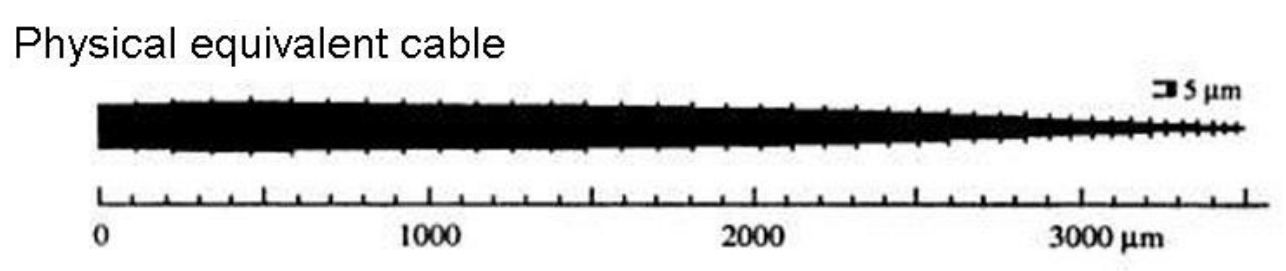
\includegraphics[scale=0.35]{03_8}
    \centering
\end{figure}
\paragraph{The Attenuation Cable}
The idea behind this approach is to disregard all the dendritic branches along which the
input signal attenuation overcomes a certain threshold: the assumption is that branches
exhibiting very fast decays are not important for the overall signal propagation.
\begin{figure}[H]
    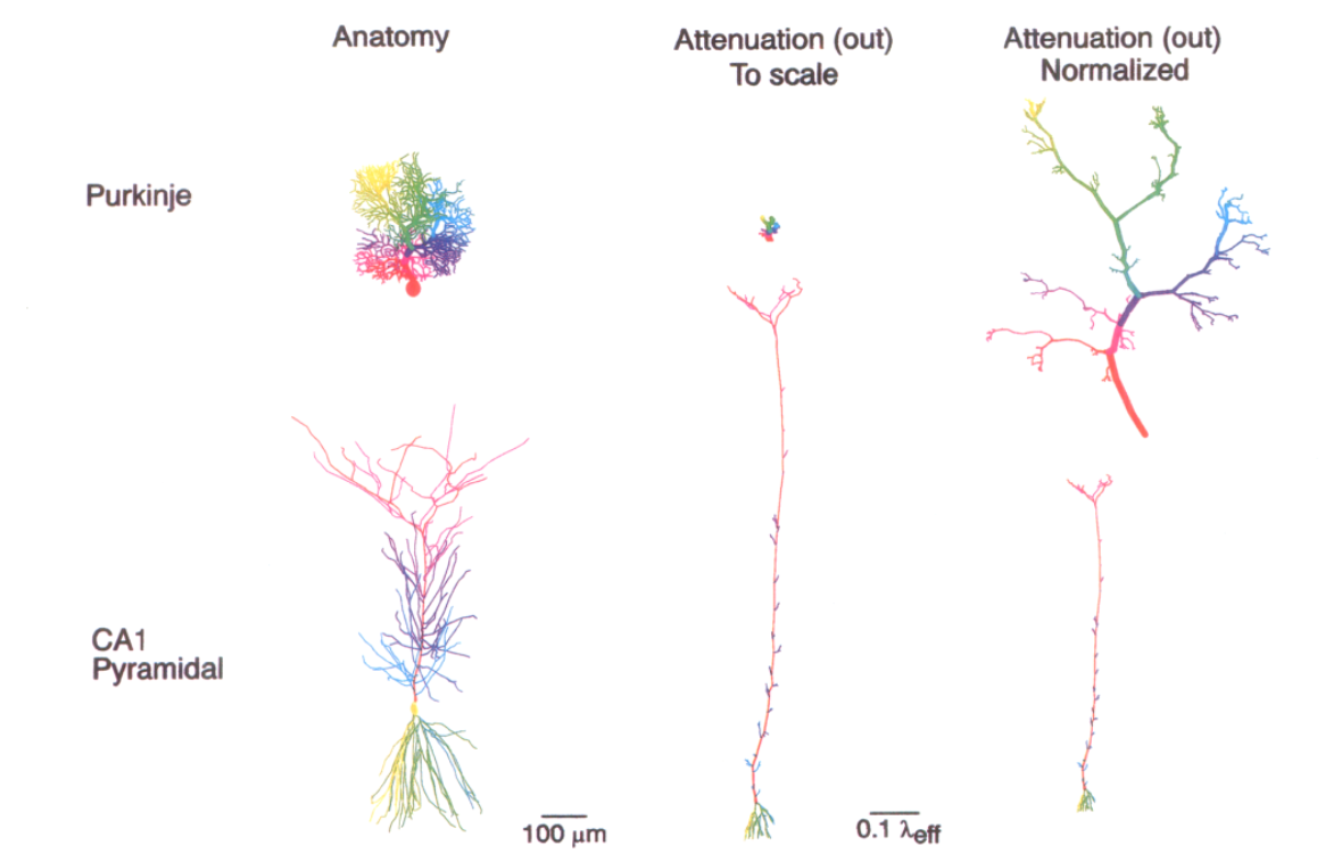
\includegraphics[scale=0.6]{03_9}
    \centering
\end{figure}
Note that the voltage attenuation is not an appropriate quantity to represent geometrically,
as it is not additive. To obtain the attenuation and delay of the membrane potential
for complex morphologies it is better to proceed as illustrated below.
\begin{figure}[H]
    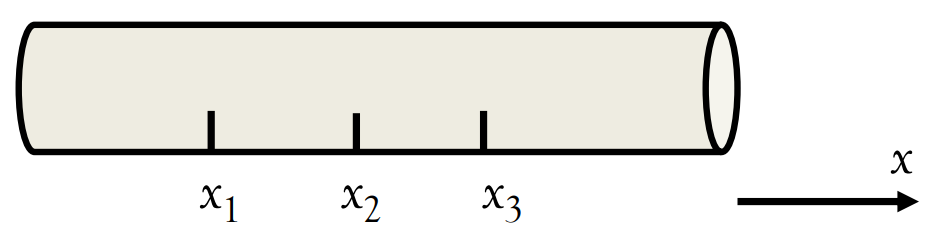
\includegraphics[scale=0.3]{03_10}
    \centering
\end{figure}
The voltage attenuation between \(x_{1}\) and \(x_{3}\) is:
\begin{equation*}
    \frac{V(x_{1})}{V(x_{3})}=\frac{V(x_{1})}{V(x_{2})}\cdot{\frac{V(x_{2})}{V(x_{3})}}
\end{equation*}
By applying the logarithm, an additive quantity is obtained, providing better information
about the signal propagation.
\begin{equation*}
    \ln{\biggl(\frac{V(x_{1})}{V(x_{3})}\biggr)}=
    \ln{\biggl(\frac{V(x_{1})}{V(x_{2})}\biggr)}+\ln{\biggl(\frac{V(x_{2})}{V(x_{3})}\biggr)}
\end{equation*}
Note that a similar approach considering signal propagation delay instead of signal
attenuation also exists.
\paragraph{The Pinsky-Rinzel 2-Comp Model}
This model is based on the fact that at least two compartments are required to properly mimic
complex patterns of electrophysiological activity. In particular, a compartment models the soma,
while another approximates the dendrites.
\begin{figure}[H]
    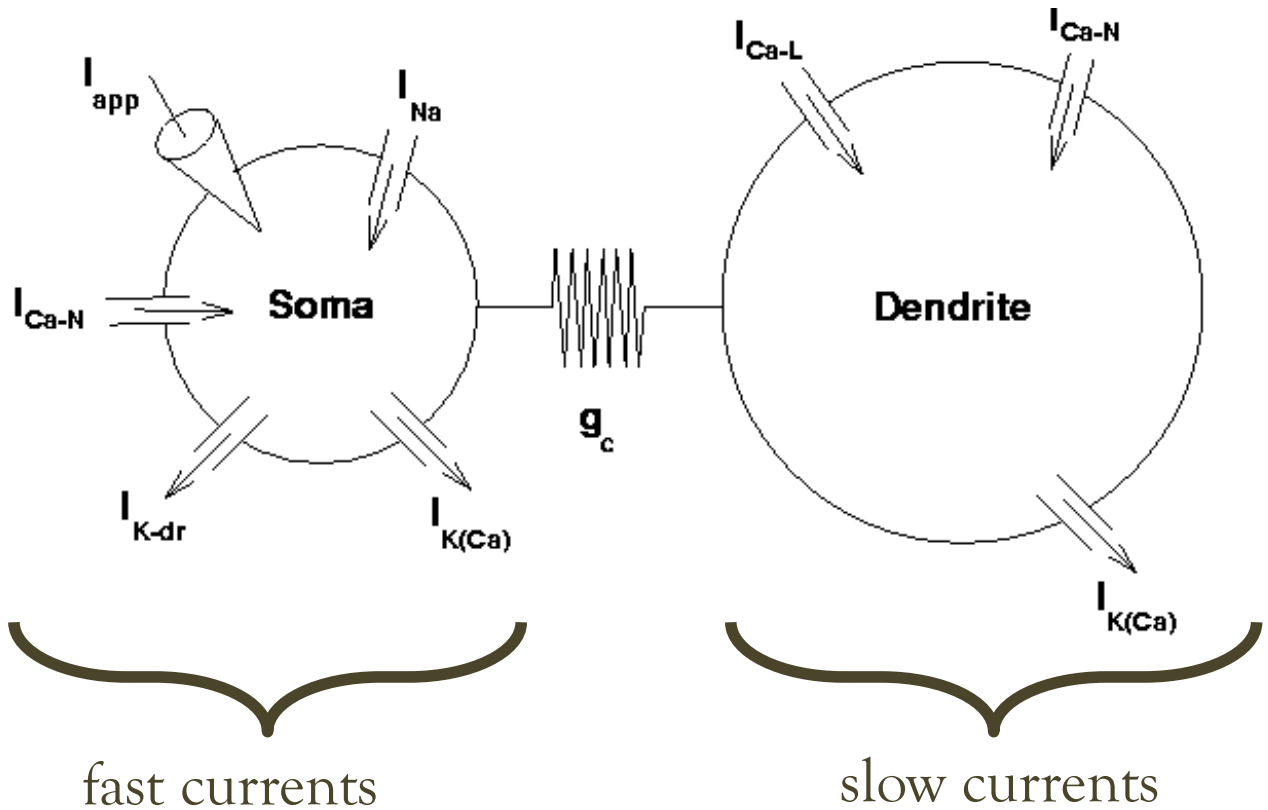
\includegraphics[scale=0.3]{03_11}
    \centering
\end{figure}
These two compartments are separated by a conductance \(g_{c}\) determining the coupling between
them, which instead regulates the kind of electrophysiological activity.
\begin{figure}[H]
    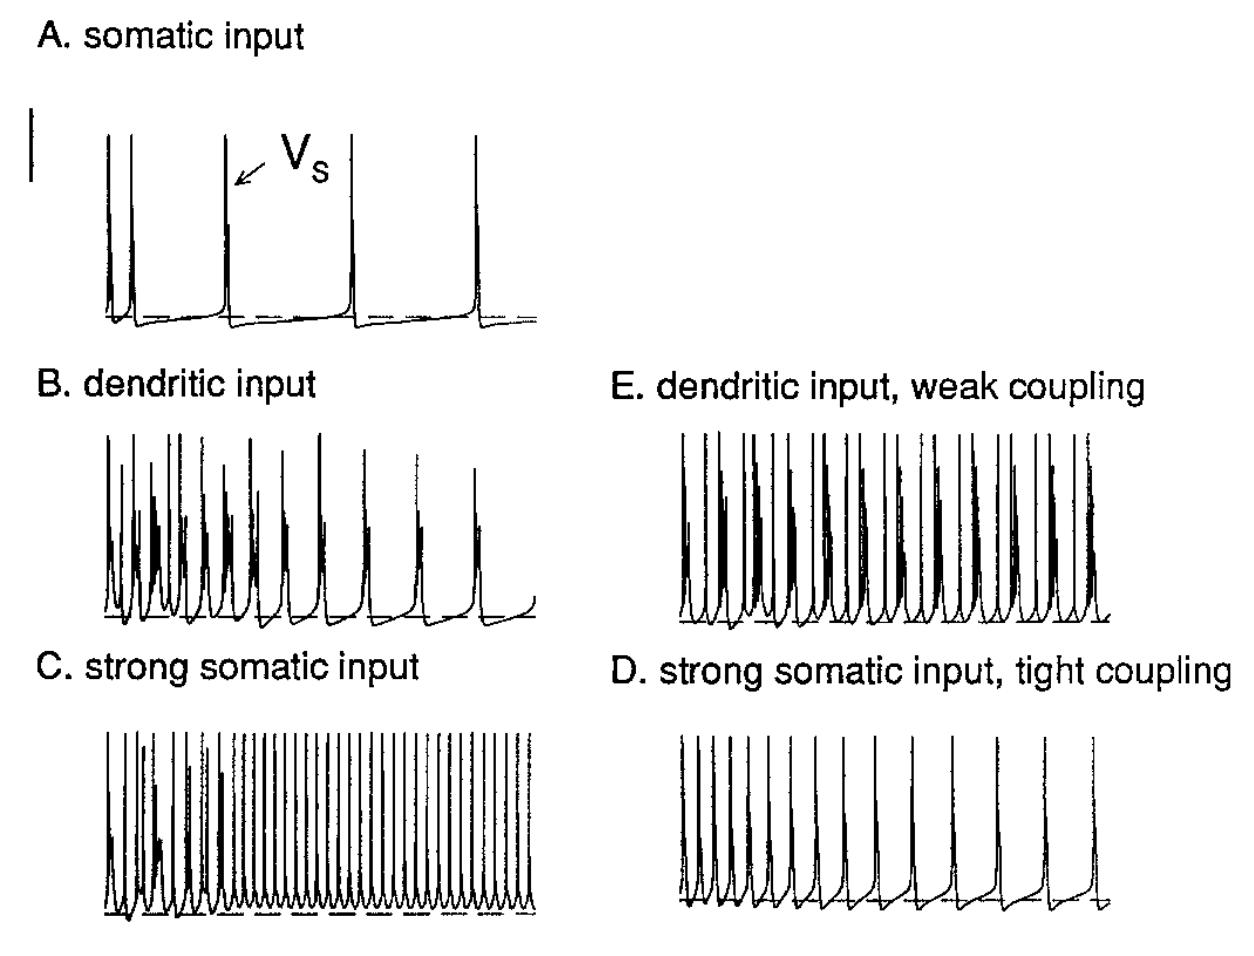
\includegraphics[scale=0.3]{03_12}
    \centering
\end{figure}

\subsection{Modelling Dendritic Spines and Synaptic Inputs}
Spines should definitely be taken into account when building the model of a neuron, they
characterize the surface of dendrites, moreover spines usually contain synapses.
\begin{figure}[H]
    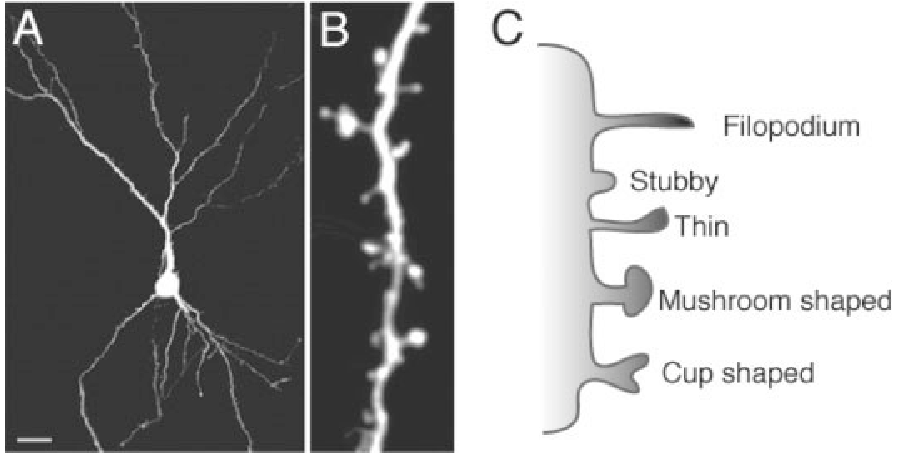
\includegraphics[scale=0.5]{03_13}
    \centering
\end{figure}
Note that several shapes are available when talking about spines, with different
geometrical properties and, as a consequence, different electrical properties.\\
When modelling spines, two distinct cases should be taken into account:
\begin{itemize}
    \item \textbf{Sipnes as \textit{passive} components}: the current flows \textit{from}
          the dendrite \textit{into} the spines.\\
          This means that spines are considered to be without synapses (no inputs). They are
          isopotential and the membrane area can be incorporated into the membrane of the parent dendrite.
          \begin{figure}[H]
              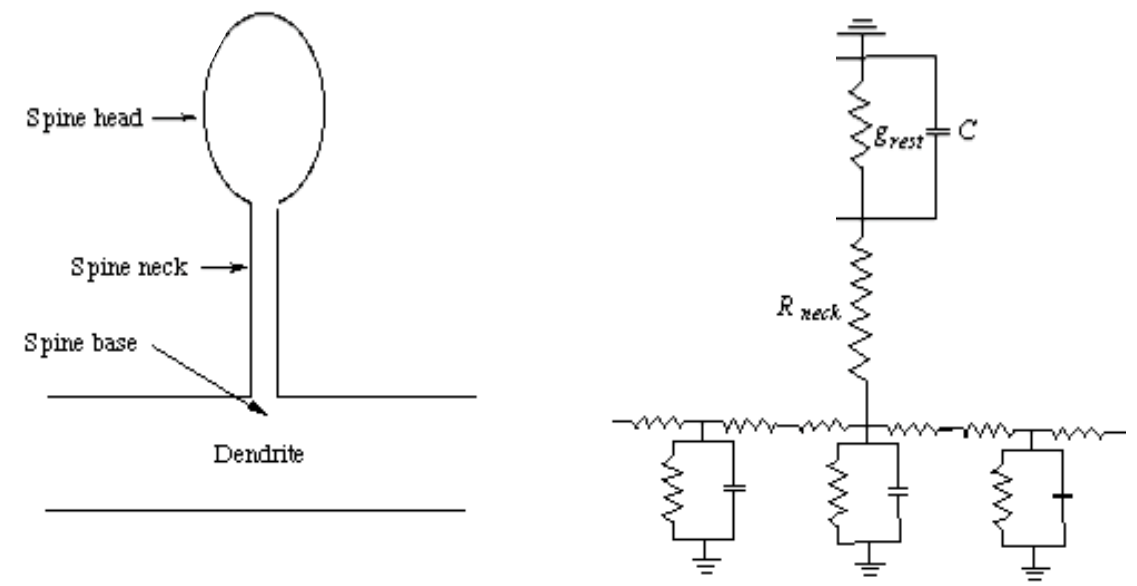
\includegraphics[scale=0.4]{03_14}
              \centering
          \end{figure}
          Both the physical dimensions and the specific membrane properties are affected by the presence
          of the spine:
          \begin{equation*}
              l'=l\cdot{F^{\frac{2}{3}}}
              \hspace{2.5cm}
              R_{m}'=\frac{R_{m}}{F}
          \end{equation*}
          \begin{equation*}
              d'=d\cdot{F^{\frac{2}{3}}}
              \hspace{2.5cm}
              C_{m}'=\frac{C_{m}}{F}
          \end{equation*}
          \begin{equation*}
              F=\frac{A_{dendrite}+A_{spine}}{A_{dendrite}}
          \end{equation*}
    \item \textbf{Sipnes as \textit{active} components}: the current is generated at the head membrane.\\
          In this case the spine contains a synapse, as an input current flows into it. The synaptic input
          can be modelled through a time-varying synaptic conductance.
          \begin{figure}[H]
              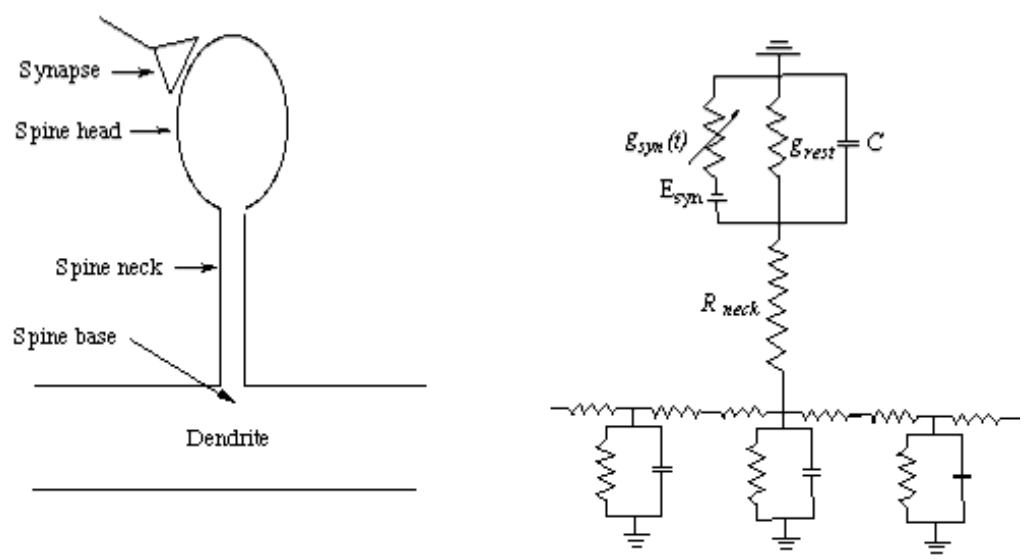
\includegraphics[scale=0.4]{03_15}
              \centering
          \end{figure}
          Here the factor \(F\) used in the
          other case can no longer be employed, as each spine exhibits its own kinetics.
\end{itemize}
\newpage

\section{Cable Theory Applied to Dendritic Structures}
\graphicspath{ {./images/04/} }
\subsection{The Cable Theory}
\subsubsection{Introduction}
The Cable Theory, first developed in 1850s and applied to neuroscience in 1930s and 1940s,
is based on a strong assumption: neuronal processes contain only voltage-independent
components. In other words, neurons are assumed to work exclusively as passive components,
therefore only resistances and capacitances are considered.\\
The following quantities represents the electrical components involved in the Cable Theory.
\begin{figure}[H]
    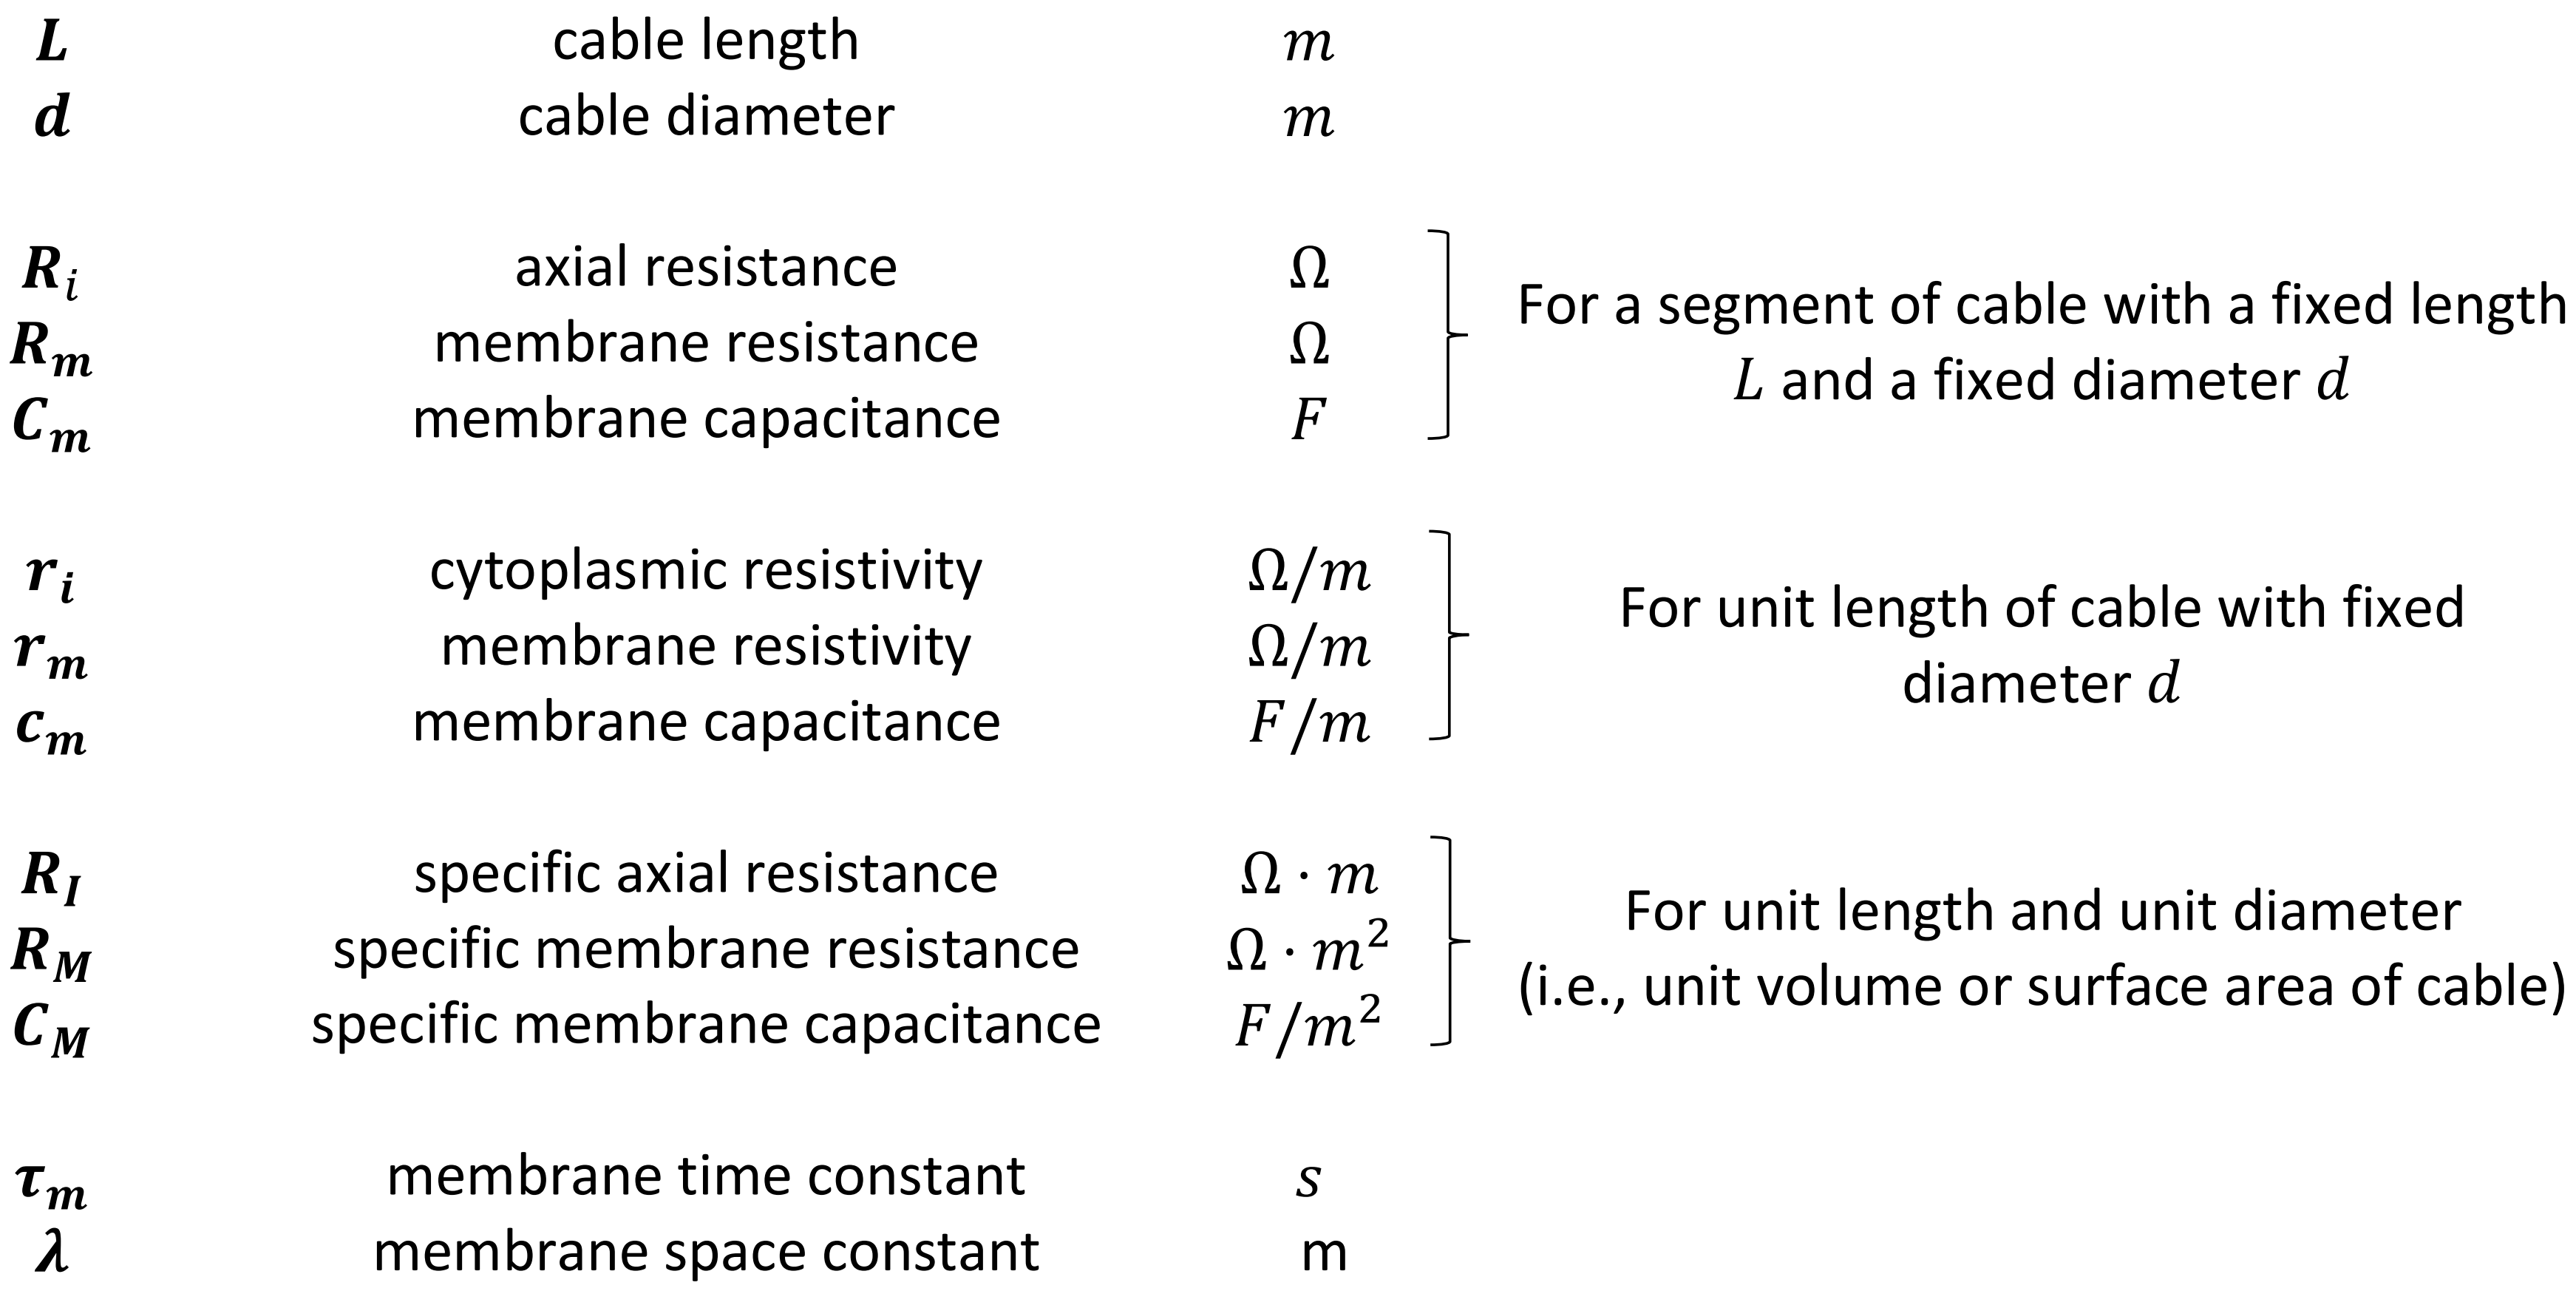
\includegraphics[scale=0.18]{04_1}
    \centering
\end{figure}
Note that given these measures, the relatonships reported here hold:
\begin{gather*}
    R_{i}=r_{i}L=\frac{4L}{\pi{d^2}}R_{I}
    \hspace{2cm}
    R_{m}=\frac{r_{m}}{L}=\frac{R_{M}}{\pi{dL}}
    \hspace{2cm}
    C_{m}=c_{m}L=\pi{dLC_{M}}\\
    \lambda=\sqrt{\frac{r_{m}}{r_{i}}}=\sqrt{\frac{d}{4}\frac{R_{M}}{R_{I}}}
    \hspace{2.5cm}
    \tau_{m}=r_{m}c_{m}=R_{M}C_{M}=R_{m}C_{m}
\end{gather*}
The cable is modelled as depicted below and the subsequent canonical expression for
the cable equation is derived.
\begin{figure}[H]
    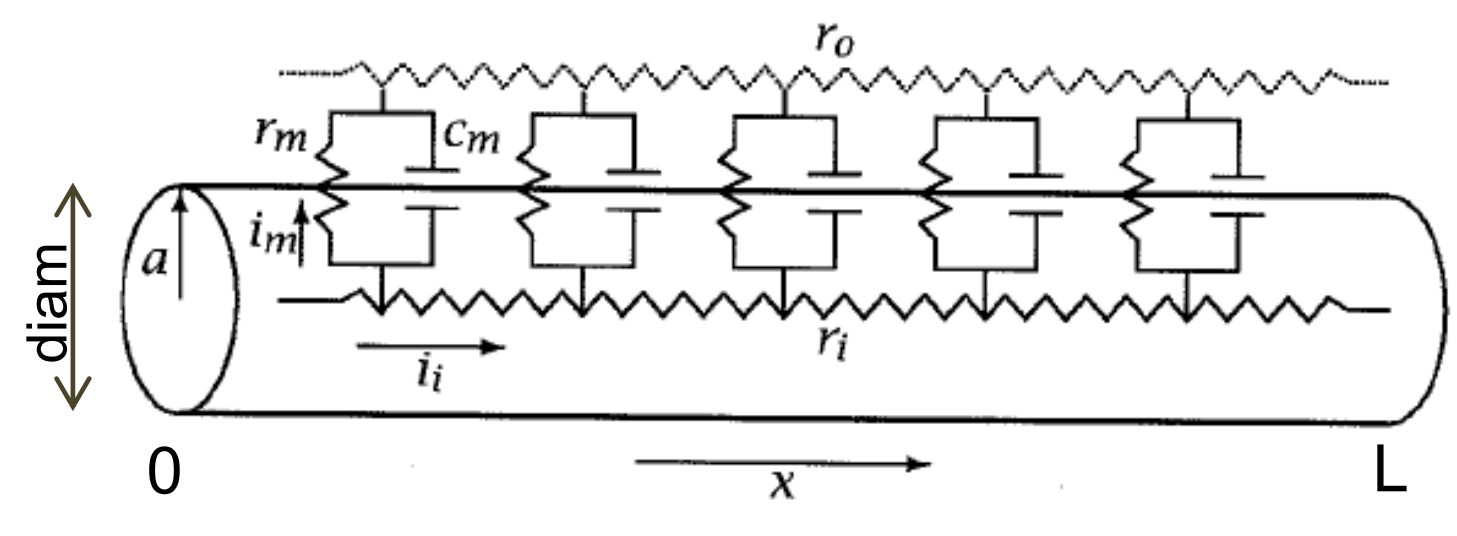
\includegraphics[scale=0.26]{04_2}
    \centering
\end{figure}
\begin{equation*}
    \lambda^{2}\frac{\partial^{2}V}{\partial{x^{2}}}-V-\tau{\frac{\partial{V}}{\partial{t}}}=0
    \Rightarrow
    \frac{\partial^{2}V}{\partial{X^{2}}}-V-\frac{\partial{V}}{\partial{T}}=0
\end{equation*}
Note that \(X=\frac{x}{\lambda}\) and \(T=\frac{t}{\tau}\), while \(V=(V_{i}-V_{e})-E_{r}\), with
\(V_i\) being the intracellular potential and \(V_e\) the extracellular one.
\subsubsection{Proof (Cable Equation Derivation)}
First of all, it is important to establish some hypotheses:
\begin{itemize}
    \item Neuronal processes contain only voltage-independent components, thus only passive
          electrical quantities are considered.
    \item The neurite is short (either axon or dendrites): \(L<\lambda\).
    \item The neurite length is much greater than its diameter: \(L>>d\).
    \item The propagation of the current is longitudinal, thus the current flows in parallel
          to the cylinder axis: \(r_{m}>>r_{i}\).
    \item The electrical properties of the membranes (\(r_{m}\), \(r_{i}\), \(c_{m}\)) are
          assumed to be uniform: \(V=V(t,x)\).
\end{itemize}
\begin{figure}[H]
    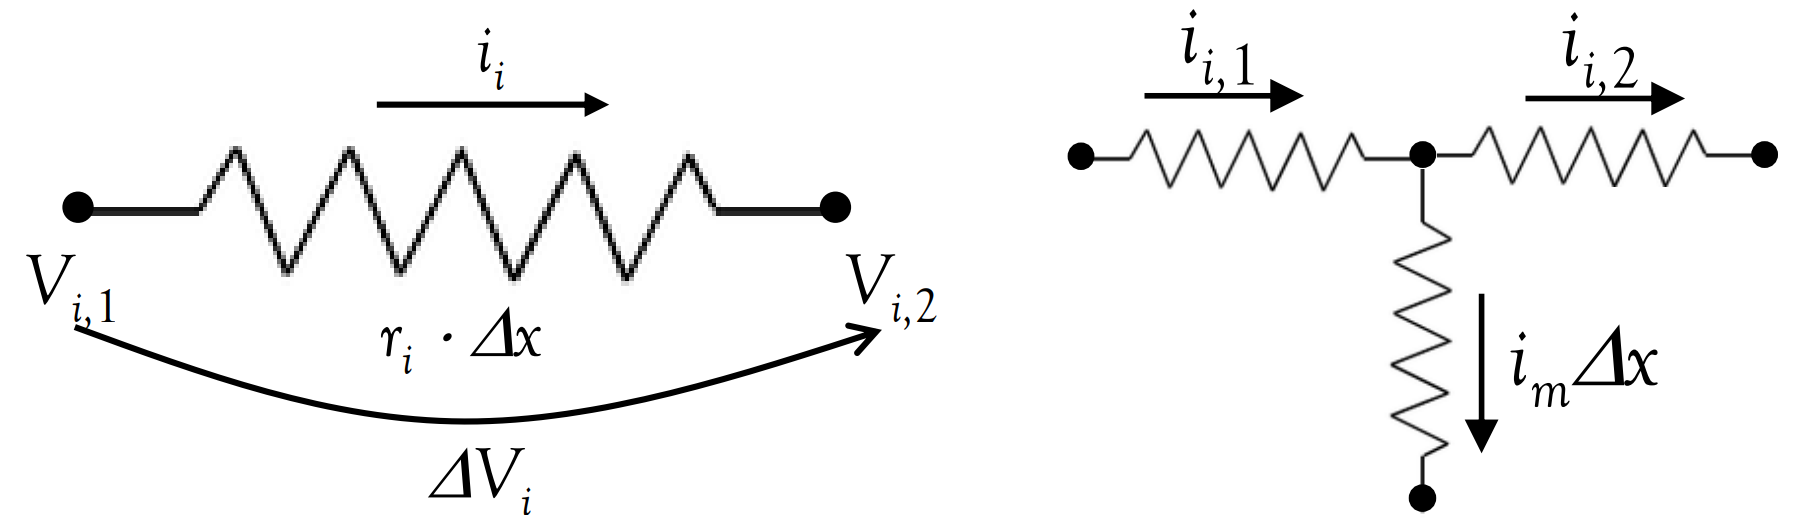
\includegraphics[scale=0.3]{04_3}
    \centering
\end{figure}
Due to the Ohm's Law:
\begin{equation*}
    i_{i}(r_{i}\Delta{x})=-\Delta{V_{i}}\Rightarrow\frac{\Delta{V_{i}}}{\Delta{x}}=-r_{i}i_{i}
\end{equation*}
Note that if \(\Delta{x}\) is infinitesimal (\(\Delta{x}\to{0}\)), this expression changes as:
\begin{equation*}
    \frac{\Delta{V_{i}}}{\Delta{x}}=-r_{i}i_{i}\Rightarrow\frac{\partial{V_{i}}}{\partial{x}}=-r_{i}i_{i}
\end{equation*}
Let's now derive the whole expression once again, without forgetting that \(r_{i}\) is uniform
by hypothesis:
\begin{equation*}
    \frac{\partial{V_{i}}}{\partial{x}}=-r_{i}i_{i}
    \Rightarrow
    \frac{\partial^{2}V_{i}}{\partial{x^{2}}}=-\frac{\partial{r_{i}i_{i}}}{\partial{x}}
    \Rightarrow
    \frac{\partial^{2}V_{i}}{\partial{x^{2}}}=-r_{i}\frac{\partial{i_{i}}}{\partial{x}}
\end{equation*}
At this point, some considerations can be done:
\begin{itemize}
    \item \(\frac{\partial{i_{i}}}{\partial{x}}=0\): there are no current variations
          within the increment \(\Delta{x}\).
    \item \(\frac{\partial{i_{i}}}{\partial{x}}<0\Rightarrow\frac{\partial^{2}V_{i}}{\partial{x^{2}}}>0\):
          there is an excess of current in the increment \(\Delta{x}\), thus an outward current \(i_{m}\) should
          be accounted for.
    \item \(\frac{\partial{i_{i}}}{\partial{x}}>0\Rightarrow\frac{\partial^{2}V_{i}}{\partial{x^{2}}}<0\):
          there is an entering current in the increment \(\Delta{x}\), indicating the presence of a synapse.
\end{itemize}
By applying the KCL, one can write that
\begin{equation*}
    i_{i,2}-i_{i,1}=-i_{m}\Delta{x}
    \Rightarrow
    \Delta{i_{i}}=-i_{m}\Delta{x}
    \Rightarrow
    -\frac{\Delta{i_{i}}}{\Delta{x}}=i_{m}
\end{equation*}
and if \(\Delta{x}\to{0}\) it becomes the following:
\begin{equation*}
    -\frac{\Delta{i_{i}}}{\Delta{x}}=i_{m}
    \Rightarrow
    -\frac{\partial{i_{i}}}{\partial{x}}=i_{m}
\end{equation*}
At this point, the resulting expression can be substituted into the previous one, leading to:
\begin{equation*}
    \frac{\partial^{2}V_{i}}{\partial{x^{2}}}=-r_{i}\frac{\partial{i_{i}}}{\partial{x}}
    \Rightarrow
    \frac{\partial^{2}V_{i}}{\partial{x^{2}}}=r_{i}i_{m}
    \Rightarrow
    \frac{1}{r_{i}}\frac{\partial^{2}V_{i}}{\partial{x^{2}}}=i_{m}
\end{equation*}
By reconsidering once again the previous hypotheses, it has been said that \(V=(V_{i}-V_{e})-E_{r}=V(x,t)\),
however the extracellular liquid is assumed to be isopotential, thus \(V_{e}\) and \(E_{r}\) are
independent on space \(x\) and time \(t\). As a consequence:
\begin{equation*}
    V=(V_{i}-V_{e})-E_{r}
    \Rightarrow
    V_{i}=V+V_{e}+E_{r}
    \Rightarrow
    \frac{\partial{V_{i}}}{\partial{x}}=\frac{\partial{V}}{\partial{x}}
\end{equation*}
Let's now take the previous equation and multiply it by \(r_{m}\):
\begin{equation*}
    \frac{1}{r_{i}}\frac{\partial^{2}V_{i}}{\partial{x^{2}}}\cdot{r_{m}}=i_{m}\cdot{r_{m}}
    \Rightarrow
    \frac{r_{m}}{r_{i}}\frac{\partial^{2}V}{\partial{x^{2}}}=r_{m}i_{m}
\end{equation*}
From now on, the \(i\)-th compartment depicted below is considered.
\begin{figure}[H]
    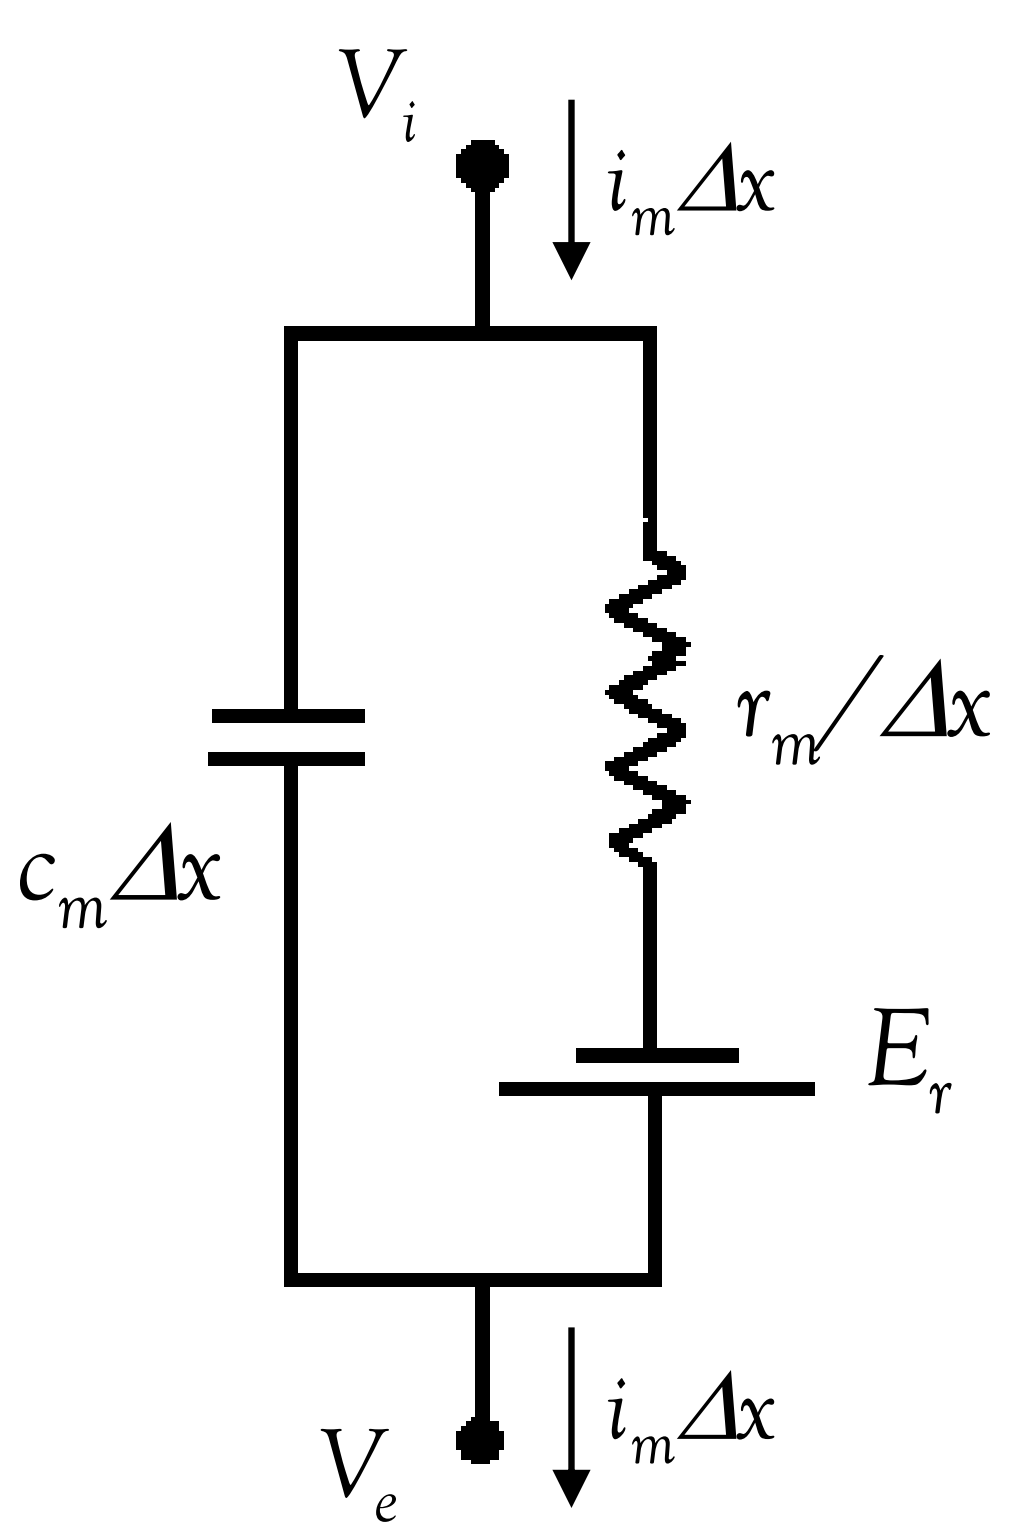
\includegraphics[scale=0.22]{04_4}
    \centering
\end{figure}
By considering its state equation, it can be said that:
\begin{equation*}
    i_{m}=c_{m}\frac{\partial{V}}{\partial{t}}+\frac{(V_{i}-V_{e})-E_{r}}{r_{m}}
    \Rightarrow
    r_{m}i_{m}=r_{m}c_{m}\frac{\partial{V}}{\partial{t}}+V
    \Rightarrow
    r_{m}i_{m}=\tau_{m}\frac{\partial{V}}{\partial{t}}+V
\end{equation*}
as the time constant is defined as \(\tau_{m}=r_{m}c_{m}\).\\
Since
\begin{equation*}
    \frac{r_{m}}{r_{i}}\frac{\partial^{2}V}{\partial{x^{2}}}=r_{m}i_{m}
    \hspace{1.5cm}
    \text{and}
    \hspace{1.5cm}
    \tau_{m}\frac{\partial{V}}{\partial{t}}+V=r_{m}i_{m}
\end{equation*}
it can be easily derived that
\begin{equation*}
    \frac{r_{m}}{r_{i}}\frac{\partial^{2}V}{\partial{x^{2}}}
    =
    \tau_{m}\frac{\partial{V}}{\partial{t}}+V
    \Rightarrow
    \lambda^{2}\frac{\partial^{2}V}{\partial{x^{2}}}-V-\tau_{m}\frac{\partial{V}}{\partial{t}}
    =
    0
\end{equation*}
with \(\lambda=\sqrt{\frac{r_{m}}{r_{i}}}\) being the space constant.
\subsubsection{Space and Time Constants}
\begin{itemize}
    \item \textbf{Space constant \(\lambda\)}: it depends not only on the axoplasmatic
          and membrane resistances (\(r_{i}\) and \(r_{m}\) respectively), but on the cable
          diameter as well, as illustrated by this relationship:
          \begin{equation*}
              \lambda=\sqrt{\frac{r_{m}}{r_{i}}}=\sqrt{\frac{R_{m}}{R_{i}}\frac{d}{4}}
          \end{equation*}
          In particular, cylinders with a bigger diameter tends to exhibit a bigger
          spatial constant, implying that the signal needs a greater distance to be attenuated.
    \item \textbf{Time constant \(\tau\)}: it defines the transient voltage response
          of a segment of the membrane to a current step input. It is formalized as:
          \begin{equation*}
              \tau=\tau_{m}=r_{m}c_{m}=R_{m}C_{m}=R_{M}C_{M}
          \end{equation*}
          Note that a bigger - i.e., slower - time constant implies a slower response to a
          changing stimulus.
\end{itemize}
Note that the \(\frac{\tau}{\lambda}\) ratio represents the time required for the voltage
across the membrane to reach \(\frac{1}{e}=0.37\) of its final value.\\
The obtained equivalent expressions
\begin{equation*}
    \lambda^{2}\frac{\partial^{2}{V}}{\partial{x^{2}}}-V-\tau\frac{\partial{V}}{\partial{t}}=0
    \hspace{2cm}
    \text{and}
    \hspace{2cm}
    \frac{\partial^{2}{V}}{\partial{X^{2}}}-V-\frac{\partial{V}}{\partial{T}}=0
\end{equation*}
are Partial Differential Equations (PDEs) and they were derived under the crucial
assumption that the axoplasmatic resistance \(r_{i}\) is uniform and constant: without this
hypothesis it is much more difficult to find a solution for the differential equation, as the
following term would change.
\begin{equation*}
    \frac{\partial^{2}V_{i}}{\partial{x^{2}}}=-r_{i}\frac{\partial{i_{i}}}{\partial{x}}
    \Rightarrow
    \frac{\partial^{2}V_{i}}{\partial{x^{2}}}=
    -r_{i}\frac{\partial{i_{i}}}{\partial{x}}-i_{i}\frac{\partial{r_{i}}}{\partial{x}}
\end{equation*}
As differential equations and time are involved, two kinds of solutions should be taken into
account:
\begin{itemize}
    \item \textbf{Steady-state solutions}
    \item \textbf{Time-dependent solutions}
\end{itemize}
\subsubsection{Cable Equation Steady-State Solutions}
In steady-state conditions, there is no change of voltage over time, therefore
the cable equation becomes an Ordinary Differential Equation (ODE):
\begin{equation*}
    \frac{\partial^{2}{V}}{\partial{X^{2}}}-V-\cancel{\frac{\partial{V}}{\partial{T}}}=0
    \Rightarrow
    \frac{\partial^{2}{V}}{\partial{X^{2}}}-V=0
\end{equation*}
The solution of such ODE can be equivalently expressed as:
\begin{itemize}
    \item \(V(X)=A_{1}e^{X}+A_{2}e^{-X}\)
    \item \(V(X)=B_{1}\cosh{(X)}+B_{2}\sinh{(X)}\)
    \item \(V(X)=C_{1}\cosh{(L-X)}+C_{2}\sinh{(L-X)}\)
\end{itemize}
where \(X=\frac{x}{\lambda}\) is the electrotonic coordinate and \(L=\frac{l}{\lambda}\)
is the electrotonic distance. Note that the solution will exhibit a sort of
expotential decay as the distance \(x\) from the input point increases.
\begin{figure}[H]
    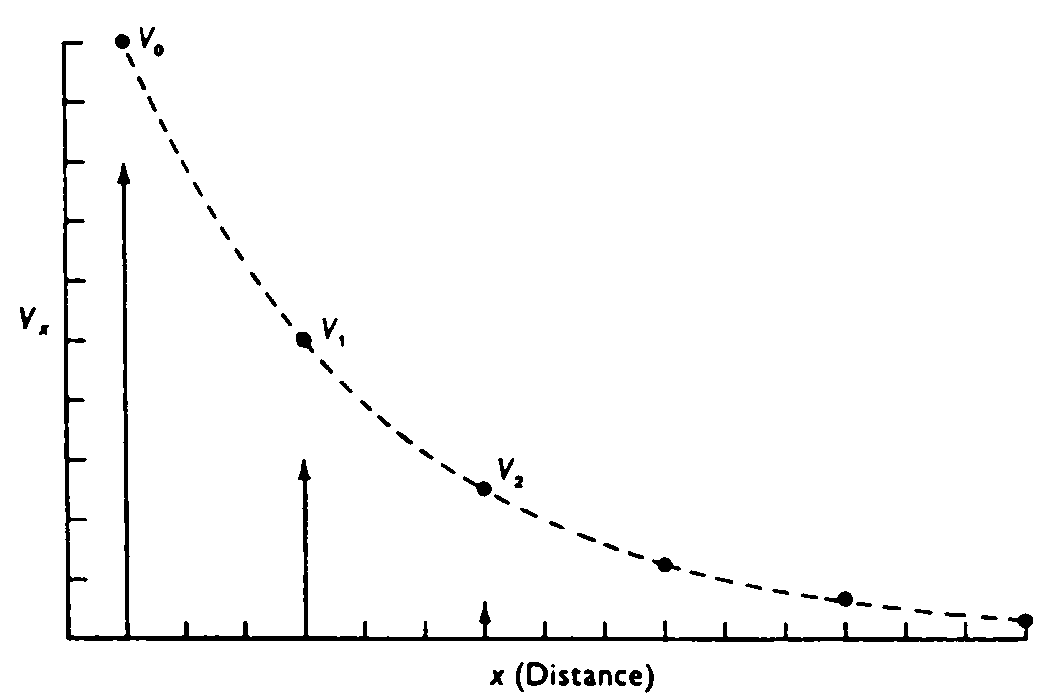
\includegraphics[scale=0.4]{04_5}
    \centering
\end{figure}
Several cases are considered in the following.
\paragraph{Semi-Infinite Cable} This model is not closed on the end side. The voltage
decays exponentially to zero as the distance from the current injection site is increased,
with a rate controlled by the space constant \(\lambda\).\\
\textit{Boundary Conditions:}
\begin{itemize}
    \item \(V(0)=V_{0}=\text{initial voltage}\)
    \item \(V(\infty)=0\)
\end{itemize}
\textit{General Solution:} \(V(X)=A_{1}e^{X}+A_{2}e^{-X}\)\\
\textit{Computations:}
\begin{gather*}
    V(X)\xrightarrow{X\to{\infty}}{0}
    \Rightarrow{0=A_{1}e^{X}+\cancelto{0}{A_{2}e^{-X}}}
    \Rightarrow{A_{1}e^{\infty}=0}
    \Rightarrow{A_{1}=0}\\
    V(X)\mid{}_{X=0}=V_{0}
    \Rightarrow{V_{0}=\cancel{A_{1}}+A_{2}}
    \Rightarrow{A_{2}=V_{0}}
\end{gather*}
\textit{Steady-State Solution:}
\begin{equation*}
    V(X)=V_{0}e^{-X}=V_{0}e^{-\frac{x}{\lambda}}
\end{equation*}
\paragraph{Finite Cable with Sealed End} The end of the cable is closed by an infinte
resistance \(R_{m}\), thus no axial current \(i_{i}\) flows at the end.\\
\textit{Boundary Conditions:}
\begin{itemize}
    \item \(V(0)=V_{0}=\text{initial voltage}\)
    \item \(i_{i}(L)=0\Rightarrow{\frac{\partial{V}}{\partial{X}}\mid{}_{X=L}=0}\)
\end{itemize}
\textit{General Solution:} \(V(X)=C_{1}\cosh{(L-X)}+C_{2}\sinh{(L-X)}\)\\
\textit{Computations:}
\begin{gather*}
    \frac{\partial{V}}{\partial{X}}\mid{}_{X=L}=0
    \Rightarrow{0=-\cancel{C_{1}\sinh{(L-L)}}-C_{2}\cosh{(L-L)}}
    \Rightarrow{0=C_{2}\cancelto{1}{\cosh{(0)}}}
    \Rightarrow{C_{2}=0}\\
    V(0)=V_{0}
    \Rightarrow{C_{1}\cosh{(L)}+\cancel{C_{2}\sinh{(L)}}}
    \Rightarrow{C_{1}=\frac{V_{0}}{\cosh{(L)}}}
\end{gather*}
\textit{Steady-State Solution:}
\begin{equation*}
    V(X)=V_{0}\frac{\cosh{(L-X)}}{\cosh{(L)}}
\end{equation*}
\paragraph{Finite Cable with Open End} This model is cut open at the end, providing
a short circuit to the ground - i.e., the extracellular potential.\\
\textit{Boundary Conditions:}
\begin{itemize}
    \item \(V(0)=V_{0}=\text{initial voltage}\)
    \item \(V(L)=0\)
\end{itemize}
\textit{General Solution:} \(V(X)=C_{1}\cosh{(L-X)}+C_{2}\sinh{(L-X)}\)\\
\textit{Computations:}
\begin{gather*}
    V(L)=0
    \Rightarrow{0=C_{1}\cancelto{1}{\cosh{(0)}}+\cancel{C_{2}\sinh{(0)}}}
    \Rightarrow{C_{1}=0}\\
    V(0)=V_{0}
    \Rightarrow{V_{0}=\cancel{C_{1}\cosh{(L)}}+C_{2}\sinh{(L)}}
    \Rightarrow{C_{2}=\frac{V_{0}}{\sinh{(L)}}}
\end{gather*}
\textit{Steady-State Solution:}
\begin{equation*}
    V(X)=V_{0}\frac{\sinh{(L-X)}}{\sinh{(L)}}
\end{equation*}
\paragraph{Finite Cable with Clamped End} The end of the cable is clamped
at an arbitrary voltage \(V_{L}\), it can be seen as a generalization of
the open end case, where \(V_{L}=0\).\\
\textit{Boundary Conditions:}
\begin{itemize}
    \item \(V(0)=V_{0}=\text{initial voltage}\)
    \item \(V(L)=V_{L}\)
\end{itemize}
\textit{General Solution:} \(V(X)=C_{1}\cosh{(L-X)}+C_{2}\sinh{(L-X)}\)\\
\textit{Computations:}
\begin{gather*}
    V(L)=V_{L}
    \Rightarrow{V_{L}=C_{1}\cancelto{1}{\cosh{(0)}}+\cancel{C_{2}\sinh{(0)}}}
    \Rightarrow{C_{1}=V_{L}}\\
    V(0)=V_{0}
    \Rightarrow{V_{0}=C_{1}\cosh{(L)}+C_{2}\sinh{(L)}}
    \Rightarrow{C_{2}=\frac{V_{L}}{\tanh{(L)}}}
\end{gather*}
\textit{Steady-State Solution:}
\begin{equation*}
    V(X)=V_{L}\cosh{(L-X)}+\frac{V_{L}}{\tanh{(L)}}\sinh{(L-X)}
\end{equation*}
All the presented steady-state solutions are presented in the plot below, showing
how the voltage drops as a function of distance.
\begin{figure}[H]
    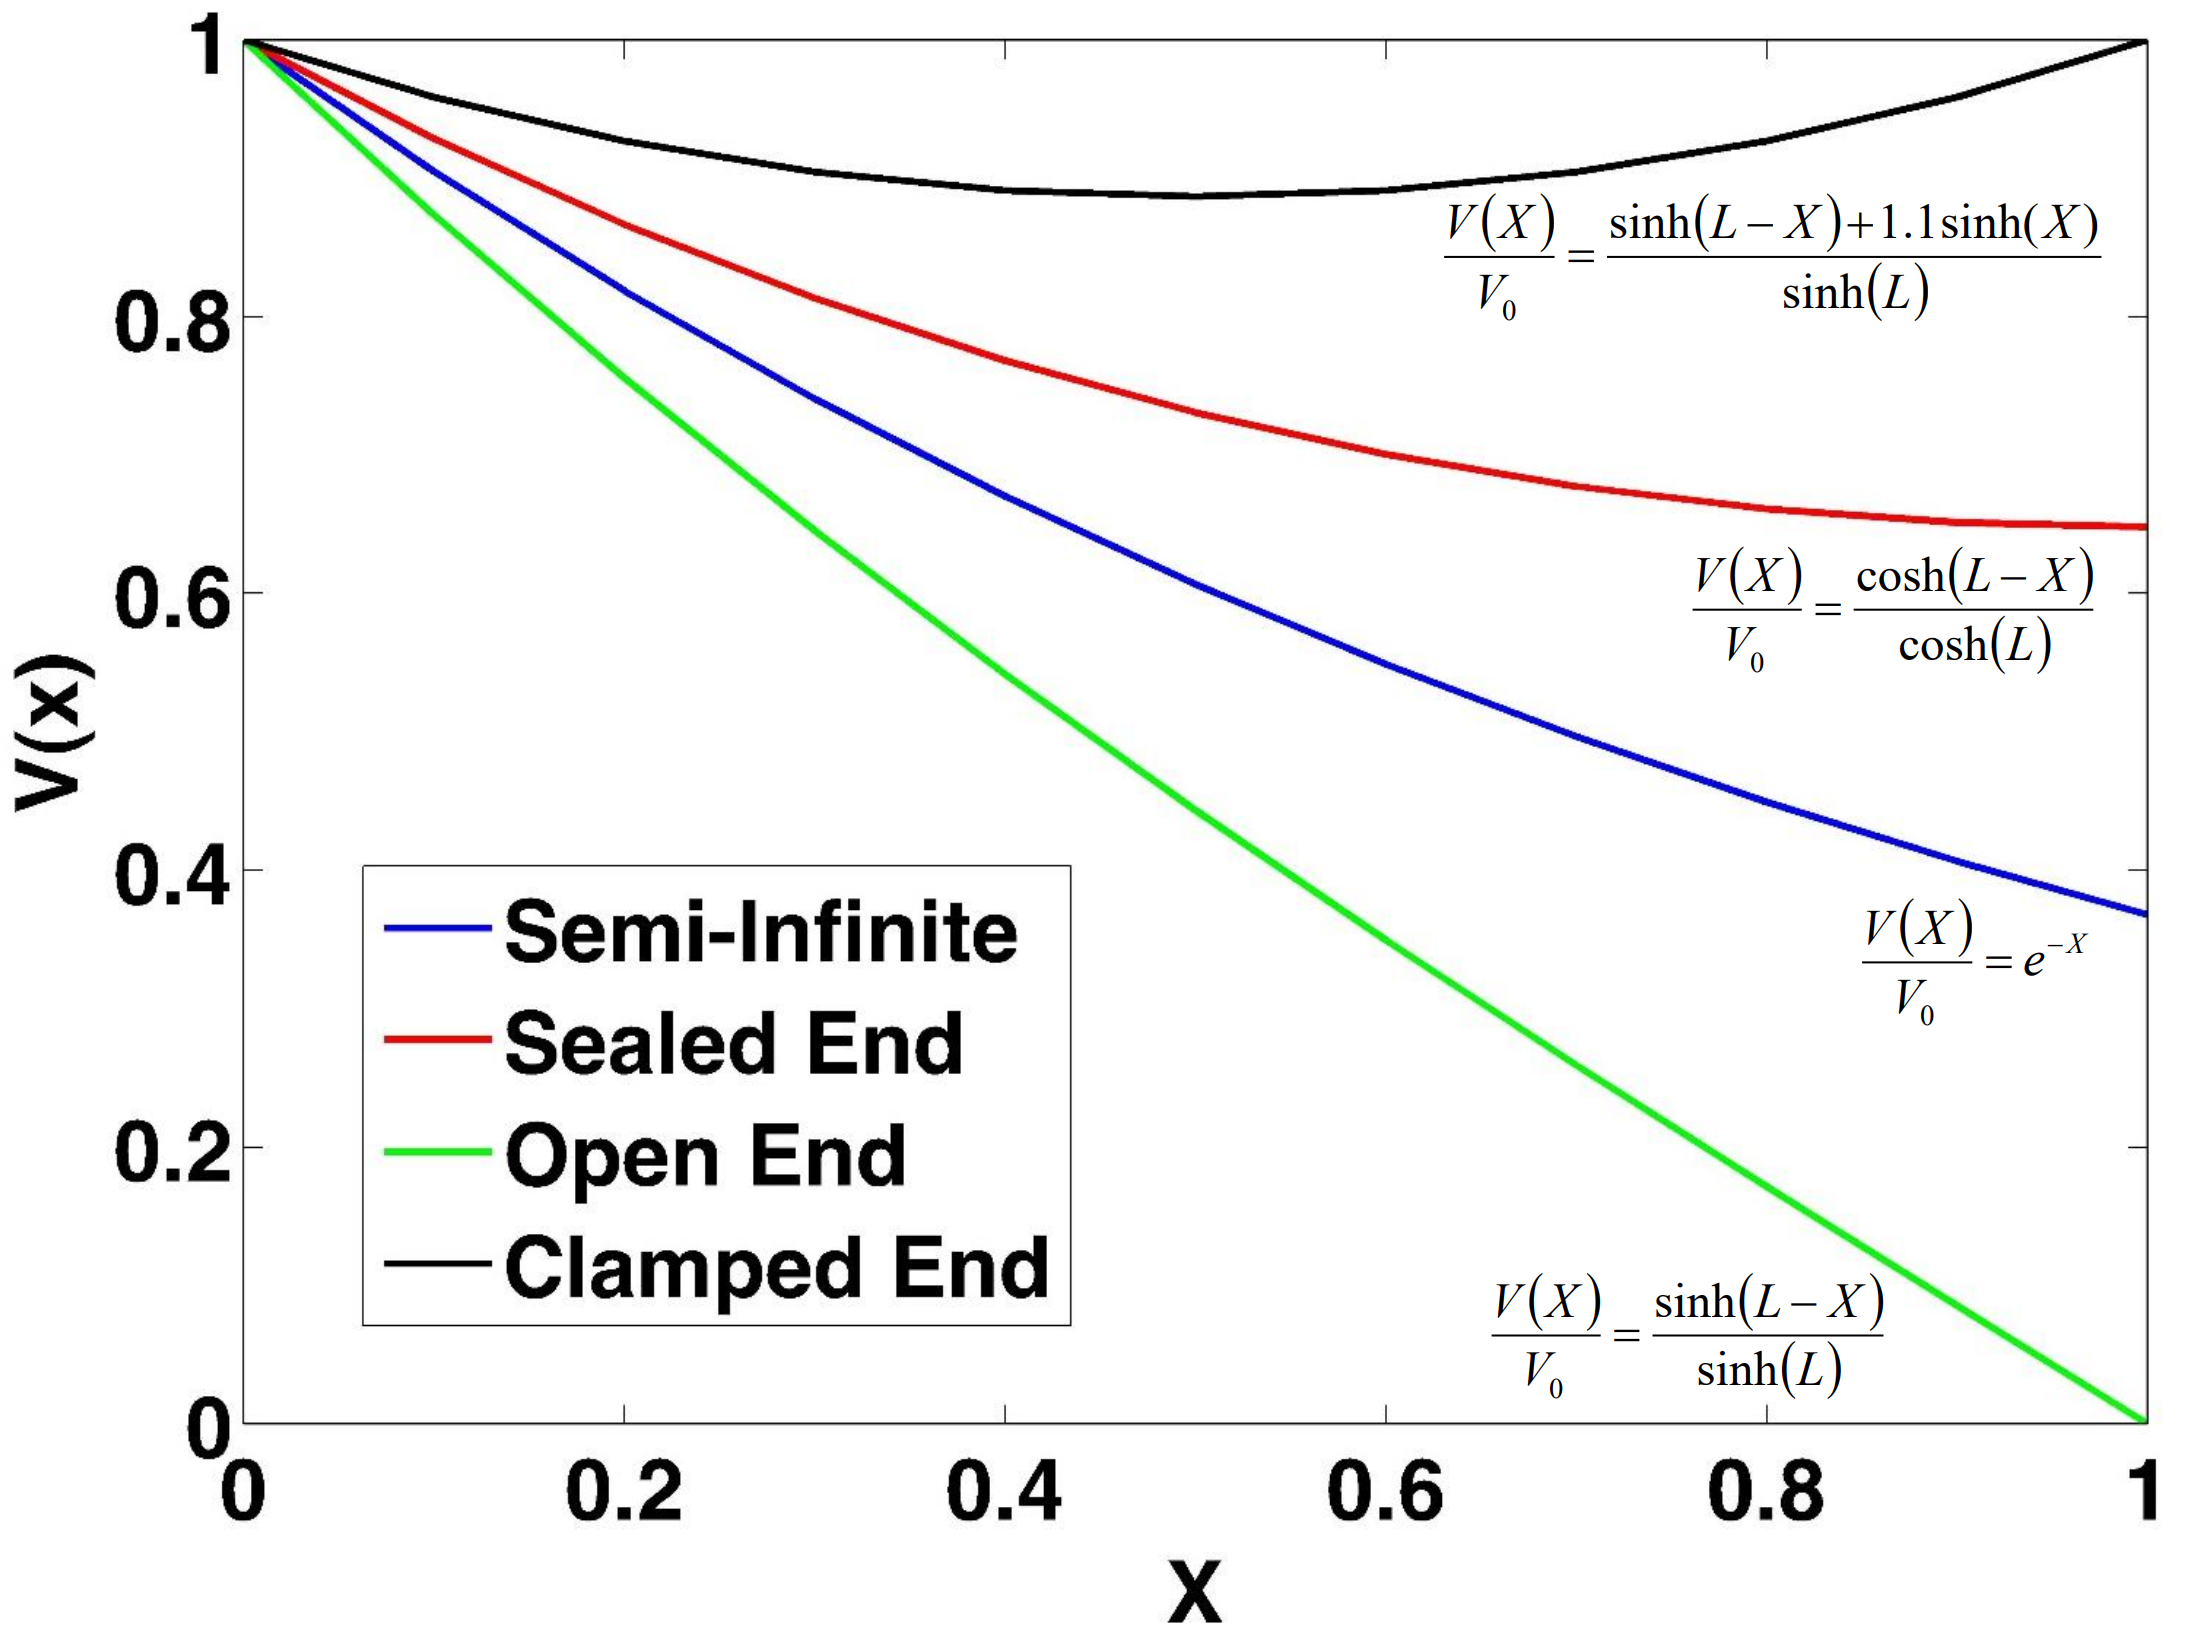
\includegraphics[scale=0.25]{04_6}
    \centering
\end{figure}
Finally, there are also two other cases of finite cable that should be taken into
account:
\begin{itemize}
    \item \textbf{Finite Cable with Leaky End}: the boundary conditions are defined
    by the same expression
    \begin{equation*}
        \pm{\frac{1}{r_{i}}\frac{\partial{V}}{\partial{x}}}\mid{}_{x=0,L}=G_{L}\cdot{V(x,t)}
    \end{equation*}
    with \(G_{L}\) being a conductance which connects the end of the cable to the resting
    potential \(E_{r}\).
    \item \textbf{Finite Cable with Current Injected at Sealed End}: the boundary conditions
    are defined by the same expression
    \begin{equation*}
        \pm{\frac{1}{r_{i}}\frac{\partial{V}}{\partial{x}}}\mid{}_{x=0,L}=I(t)
    \end{equation*}
\end{itemize}
Notice that this is used to model a dendrite stimulated from one extremity to the other
and vice-versa, in order to obtain information on the dendrite properties (collision test).
\subsubsection{Cable Equation Time-Dependent Solutions}
Firstly, let's make an hypothesis: the membrane potential is isopotential, thus it
is constant across the space, in other words \(\frac{\partial{V}}{\partial{X}}=0\).
Said so, the cable equation is simplified as follow:
\begin{equation*}
    \cancel{\frac{\partial^{2}{V}}{\partial{X^{2}}}}-V-\frac{\partial{V}}{\partial{T}}=0
    \Rightarrow
    \frac{\partial^{2}{V}}{\partial{T^{2}}}+V=0
\end{equation*}
If an isopotential neuron is stimulated by a current pulse \(I_{0}\), then:
\begin{equation*}
    V(T)=I_{0}R_{m}(1-e^{-T})
\end{equation*}
where \(R_{m}\) is the membrane resistance of the isopotential segment.\\
Whenever the stimulus is removed, the voltage decays exponentially from
its maximum value \(V(t_{0})=V_{0}\):
\begin{equation*}
    V(T)=V_{0}e^{-T}=V_{0}e^{-\frac{t}{\tau}}
\end{equation*}
In the general case of passive cylinders, thus considering both space and
time constants, the solution of the cable equation \(V(X,T)\) can be expressed as
a sum of an infinite number of exponential decays.

\subsection{The Computational Properties of Dendrites}
When talking about dendrites one may ask whether they are somehow
important from the functional point of view or, on the other hand,
if they play only a key role in forming connections, without any
contribution in computations. With respect to how the brain process
information there are two main viewpoints:
\begin{itemize}
    \item Information processing results primarily from the properties of
    synapses and the connectivity of neurons. The contribution of a single
    neuron is negligible, the emphasis is on the complexity of the overall
    network.
    \item The focus should be on the neuron, playing a fundamental role in the
    computations, thanks to its complex morphology.
\end{itemize}
This second viewpoint is a little old-fashioned nowadays, as it was at the base
of the perceptrons, which aimed at describing the biological neurons and their
computational capabilities in a comprehensive way. The idea was that neurons are
able to operate as devices where analog computations are at a certain point
transformed into a digital output signal.\\
However, today it is mostly believed that linear and non-linear mechanisms
in the dendritic tree are likely to serve as computational building blocks:
combined together they play a key role in the overall computation performed
by a neuron.
\subsubsection{Passive Dendrites}
\paragraph{Passive Filters} They may act as linear filters acting on the input signal: this
kind of filtering tends to attenuate the dendritic signal as a function of the travelled
distance and its frequency. As a consequence, if a signal is too low in power or very
far away it tends to be disregarded.
\paragraph{Non-linear Interactions} Whenever excitatory and inhibitory inputs are
widely separated from one another on different dendritic branches, the input signals
will tend to sum linearly at the soma (a logic OR).\\
If the inputs are adjacent to each other the inhibition can produce a highly non-linear
shunting of the excitatory input (a logic AND-NOT).\\
Moreover, the branch points in the dendritic tree sums up the currents in individual
branches.
\paragraph{Reducing and Amplifying the Mutual Interaction} Generally, excitatory
inputs to the same branch tend to sum sublinearly, whereas inputs on different branches
sum linearly.
\paragraph{Coincidence Detection} The back-propagation of action potentials triggers
a dendritic Ca\({}^{2+}\) spike which depolarizes the whole apical dendrite and drives
a burst of spikes in the axon.
\begin{figure}[H]
    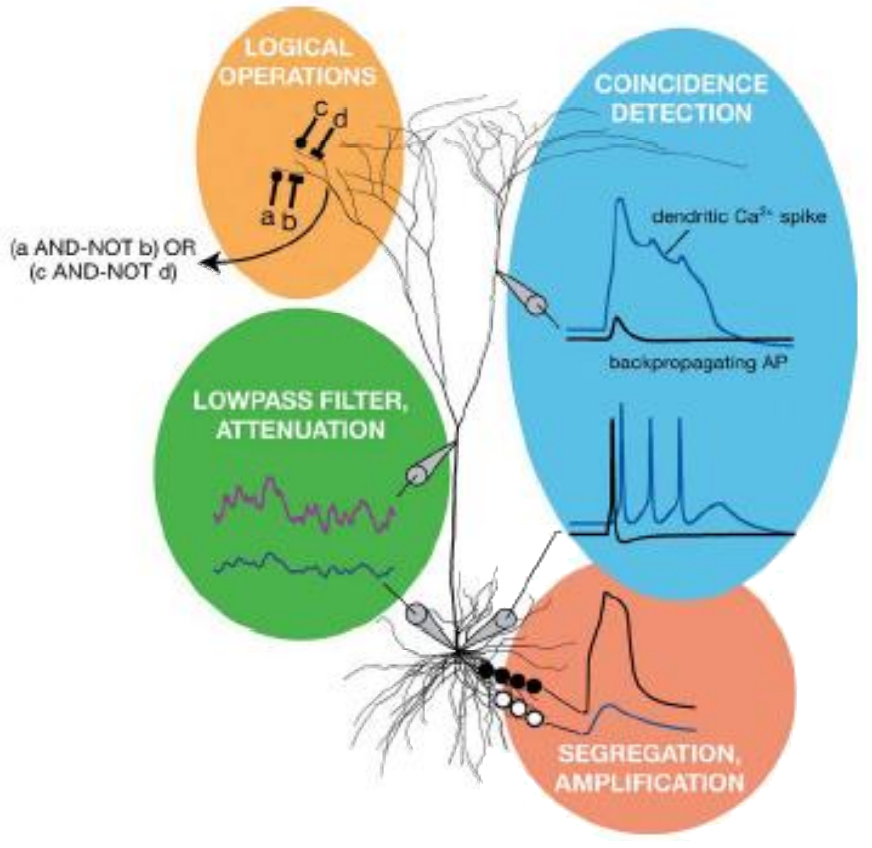
\includegraphics[scale=0.5]{04_7}
    \centering
\end{figure}
\subsubsection{Active Dendrites}
\paragraph{Dynamic Polarization Law} In the nervous system information flows in one
direction, from dendrites to the soma and then to the axon.
\paragraph{Back-propagation Theory} The presence of excitable ionic currents in the
dendrites supports dendritic action potentials that travel in the reverse direction
w.r.t. the main one. Therefore, the neuron is no longer considered to be an
open-loop system, but it presents an internal feedback mechanism.\\
In general, the amount of input is critical in defining the direction of
propagation, while the kind of computation performed is a consequence of
the dendritic tree morphology.
\newpage

\end{document}